\documentclass[11pt,final,hidelinks]{article}
\usepackage{lmodern}
\usepackage[T1]{fontenc}
\usepackage[english]{babel}
\usepackage[utf8]{inputenc}
\usepackage[activate={true,nocompatibility},final,tracking=true,kerning=true,
    spacing=true,factor=1100,stretch=10,shrink=10]{microtype}
\microtypecontext{spacing=nonfrench}
\usepackage[margin=1in]{geometry}
\usepackage{graphicx}
\graphicspath{{img/}}
\usepackage[noend]{algorithm2e}
\usepackage{caption}
\usepackage{subcaption}
\usepackage{booktabs}
\usepackage{array}
\usepackage{mathtools}
\usepackage{enumitem}
\usepackage{commath}
\usepackage{appendix}
\renewcommand\appendixtocname{Appendices}
\usepackage{amsmath}
\usepackage{amsthm}
\usepackage{amssymb}
%\usepackage[intoc,english]{nomencl}
%\makenomenclature
\usepackage{pgfplots}
\usepackage{tabu}
\usepackage{tikz}
\usepackage{tikzscale}
\usepackage[square,numbers]{natbib}
\bibliographystyle{plain}
\usepackage{siunitx}
\numberwithin{equation}{section}
\usepackage{hyperref}
\usepackage{cleveref}

\pgfplotsset{compat=newest}

\usepackage[fancy,section]{alex}

\hypersetup{
    pdftitle={Bernoulli sets and their corresponding random binary classification measures.},
    pdfauthor={Alexander Towell},               % author
    pdfsubject={computer science},              % subject of the %document
    pdfkeywords={
        probabilistic data structure,
        abstract data type,
        approximate set,
        bloom filter,
        perfect hash function,
        perfect hash filter},                   % keywords
    colorlinks=true,                            % false: boxed links;
    linkcolor=magenta,
    citecolor=green,                            % color of links to
    filecolor=blue,                             % color of file links
    urlcolor=green                              % color of external
}

\title
{
    Bernoulli sets: a model for modeling sets with random errors\\
    \large and corresponding random binary classification measures.
}
\author
{
    Alexander Towell\\
    \texttt{atowell@siue.edu}
}
\date{}

\begin{document}
\maketitle
\begin{abstract}
We introduce the \emph{Bernoulli set model}, a compositionally closed probabilistic framework for \emph{random approximate sets}---sets that approximate an objective set with independent, element-wise errors parameterized by false positive and false negative rates.
The central property of the model is \emph{closure}: every set-theoretic operation (complement, union, intersection, difference) on Bernoulli sets yields a Bernoulli set whose error rates are computable from the operands, and this closure extends to higher-order compositions.
From two axioms---element-wise independence and conditional independence of error rates---we derive the probability distributions of all standard binary classification measures (precision, recall, etc.), the joint entropy of error counts, and conditions under which approximate sets form commutative monoids.
The framework unifies the analysis of probabilistic data structures such as Bloom filters and perfect hash filters: any implementation satisfying the Bernoulli axioms inherits the full theory as an abstract data type.
We demonstrate this compositionality through an application to encrypted Boolean search, where showing that result sets are Bernoulli sets immediately yields all performance guarantees.
\end{abstract}

\microtypesetup{protrusion=false}
\tableofcontents
\microtypesetup{protrusion=true}

%%%%%%%%%%%%%%%%%%%%%%%%%%%%%%%%
% Introduction
%%%%%%%%%%%%%%%%%%%%%%%%%%%%%%%%

\section{Introduction}

Many computational systems rely on \emph{approximate set representations}---data structures whose membership queries may err, returning false positives or false negatives with known rates.
Bloom filters~\cite{bf}, perfect hash filters~\cite{phf}, and related probabilistic data structures achieve dramatic space savings by tolerating such errors, and individual structures are well understood.
However, practical systems rarely use a single approximate set in isolation.
Encrypted search indexes, database query planners, and distributed systems routinely compose approximate sets through union, intersection, complement, and difference, and the resulting error behavior has traditionally been analyzed on a case-by-case basis.

\paragraph{The gap.}
The existing literature lacks a \emph{compositional algebra} for approximate sets: a framework in which the error rates of any set-theoretic expression are mechanically computable from the error rates of its operands.
Without such a framework, each new combination of approximate sets requires a bespoke analysis, and higher-order compositions---approximate sets of approximate sets---remain largely uncharacterized.

\paragraph{Contribution.}
We introduce the \emph{Bernoulli set model}, a probabilistic framework for \emph{random approximate sets} built on two axioms: element-wise independence of errors and conditional independence of block error rates.
From these axioms we derive:
\begin{enumerate}[nosep]
    \item the binomial distributions of error counts (false positives, false negatives, true positives, true negatives) and their asymptotic normal limits,
    \item the higher-order composition theorem: the $k$-fold composition of approximate identity functions yields a Bernoulli set whose rates are given by the product of binary channel transition matrices, and
    \item confidence intervals for the realized false positive and true positive rates.
\end{enumerate}
The framework is formulated as an abstract data type: any implementation whose membership queries satisfy the Bernoulli axioms---including Bloom filters, perfect hash filters, and their compositions---inherits the full theory automatically.

\paragraph{Related work.}
The original Bloom filter~\cite{bf} introduced approximate set membership with one-sided error.
Subsequent work has produced a rich family of probabilistic data structures---including cuckoo filters~\cite{cuckooFilter}, quotient filters~\cite{quotientFilter}, xor filters~\cite{xorFilter}, and ribbon filters~\cite{ribbonFilter}---surveyed by Broder and Mitzenmacher~\cite{broderMitzenmacher}, with improved space efficiency or additional functionality.
Bose et al.~\cite{boseBloom} give tight bounds on the Bloom filter false positive rate, Kirsch and Mitzenmacher~\cite{kirschMitzenmacher} show that two hash functions suffice, and Carter and Wegman~\cite{carterWegman} provide the universal hash families underlying many implementations.
Related probabilistic summaries such as the count-min sketch~\cite{countMinSketch} trade exact answers for space efficiency in the streaming setting.
However, analyses typically treat each structure in isolation, deriving error rates for a single filter rather than for compositions of filters.
General probabilistic methods for randomized algorithms~\cite{mitzenmacherUpfal} provide the analytical toolkit (concentration inequalities, entropy bounds) but do not address the compositional structure of approximate sets.
Our framework complements these lines of work by providing an algebraic layer that sits above any particular implementation; the interval arithmetic extension for uncertain rate parameters is developed in~\cite{bernoulliComposition}.

\paragraph{Companion papers.}
The set-theoretic composition of Bernoulli sets---closed-form error rates for complement, union, intersection, and set difference, monoidal structure, relational predicates, and interval arithmetic---is developed in a companion paper~\cite{bernoulliComposition}.
The probability distributions of binary classification measures (precision, recall, accuracy, etc.) induced by the Bernoulli model are derived in~\cite{bernoulliMeasures}.
The joint entropy of error counts and the information-theoretic space complexity of approximate sets are developed in~\cite{bernoulliEntropy}.

\paragraph{Organization.}
\Cref{sec:setalgebra} reviews the algebra of sets.
\Cref{sec:bernoulli_model} introduces the Bernoulli set model and its axioms, including the higher-order composition theorem.
\Cref{sec:characteristics} derives the binomial distributions of error counts and their asymptotic normal limits.

%%%%%%%%%%%%%%%%%%%%%%%%%%%%%%%
% Algebra of sets
%%%%%%%%%%%%%%%%%%%%%%%%%%%%%%%

\section{Algebra of sets} 
\label{sec:setalgebra}
A \emph{set} is an unordered collection of distinct elements.
If we know the elements in a set, we may denote the set by these elements, e.g., $\{a,c,b\}$ denotes a set whose members are exactly $a$, $b$, and $c$.

Two sets of particular importance are the empty set, denoted by $\emptyset$, which has no members, and the \emph{universal set}, in which every element of interest is a member.

The \emph{cardinality} of a finite set $A$ is the number of elements in $A$, denoted by $|A|$.
A \emph{countably infinite set} is one that can be put into bijection with $\mathbb{N} = \{1,2,\ldots\}$.
We assume familiarity with standard set-theoretic notation (ordered pairs, Cartesian products, relations, functions); see Feller~\cite{feller} for background.

The \emph{power set} of $A$, denoted by $\mathcal{P}(A)$, is the set of all subsets of $A$.
The \emph{indicator function} of $A$ with respect to a universal set $X$ is
\begin{equation}
	\mathbf{1}_A : X \to \{0,1\}, \quad
	\mathbf{1}_A(x) =
	\begin{cases}
		1 & \text{if $x \in A$},\\
		0 & \text{if $x \notin A$}.
	\end{cases}
\end{equation}
The standard set operations---\emph{union} $A \cup B = \{x : x \in A \lor x \in B\}$, \emph{intersection} $A \cap B = \{x : x \in A \land x \in B\}$, and \emph{complement} $A^c = \{x \in X : x \notin A\}$---are used throughout.
Sets $A$ and $B$ are \emph{disjoint} if $A \cap B = \emptyset$.

\subsection{Approximate sets}
\label{sec:asets}
Given an objective set $A$, any element that is a member of $A$ is denoted a \emph{positive} (of $A$) and otherwise the element is denoted a \emph{negative}.
We write $\hat{A}$ for an arbitrary approximation of $A$; in \cref{sec:bernoulli_model}, this will be refined to the Bernoulli set $\tilde{A}$, which satisfies additional axioms.
Suppose $\hat{A}$ is used as an \emph{approximation} of $A$.
If the \emph{only} information we have about $A$ is given by $\hat{A}$, then we may perform membership tests on $\hat{A}$ to make \emph{predictions} or \emph{estimations} about $A$.

There are two ways a binary prediction can be false.
\begin{enumerate}
	\item A \emph{false positive} occurs if a negative of the objective set is predicted to be a positive. False positives are also known as \emph{type I errors}.
	The complement of false positives are \emph{true negatives}.
	\item A \emph{false negative} occurs if a positive of the objective set is predicted to be a negative. False negatives are also known as \emph{type II errors}.
	The complement of false negatives are \emph{true positives}.
\end{enumerate} 

If we denote the set of false positives by $FP$, true positives by $TP$, false negatives by $FN$, and true negatives by $TN$, then the objective set $A = FN \cup TP$ and the approximate set $\hat{A} = TP \cup FP$.
See \cref{fig:ex_approx_set} for an illustration.
\begin{figure}[ht]
	\centering
	\def\svgwidth{\columnwidth/4}
	\input{img/aset_fp_fn.tex}
	\caption{An approximate set $\hat{A}$ of an objective set $A$}
	\label{fig:ex_approx_set}
\end{figure}

If we only have access to the approximation $\hat{A}$, we do not have the ability to partition the universe into the disjoint sets $FP$, $TP$, $FN$, and $TN$ as demonstrated in \cref{fig:ex_approx_set}.
However, we can quantify the degree of \emph{uncertainty} about the elements that it predicts to be positive or negative.
The false positive and true negative rates are given by the following.
\begin{definition}
	\label{def:fprate}
	The \emph{false positive rate} is the proportion of predictions that are \emph{false positives} as given by
	\begin{equation}
	\hat{\alpha} = \frac{|FP|}{|FP| + |TN|}
	\end{equation}
	and the \emph{true negative rate} is given by $\hat{\tnrate} = 1 - \hat{\alpha}$.
\end{definition}
The true positive and false negative rates are given by the following.
\begin{definition}
	The \emph{true positive rate} is the proportion of predictions that are \emph{true positives} as given by
	\begin{equation}
	\hat{\tprate} = \frac{|TP|}{|TP| + |FN|}
	\end{equation}
	and the \emph{false negative rate} is given by $\hat{\beta} = 1 - \hat{\tprate}$.
\end{definition}

The \emph{probabilities} of the four possible predictive outcomes are given by 
\cref{tbl:contingency_table}.
\begin{table}[ht]
	\centering
	\begin{tabular}{@{} l l l @{}}
		\toprule
		& \textbf{positive} & \textbf{negative}\\
		\midrule
		\textbf{predict positive} & $\hat{\tprate}=1-\hat{\beta}$ & 
		$\hat{\alpha}=1-\hat{\tnrate}$\\
		\textbf{predict negative} & $\hat{\beta}=1-\hat{\tprate}$ & 
		$\hat{\tnrate}=1-\hat{\alpha}$\\
		\bottomrule
	\end{tabular}
	\caption{The $2 \times 2$ contingency table of outcomes for approximate sets.}
	\label{tbl:contingency_table}        
\end{table}

%%%%%%%%%%%%%%%%%%%%%%%%%%%%%%%%%
% Bernoulli model
%%%%%%%%%%%%%%%%%%%%%%%%%%%%%%%%%

\section{Bernoulli set model}
\label{sec:bernoulli_model}
In the \emph{Bernoulli} set model, we describe the statistical properties of processes that \emph{generate} approximations of a certain kind that model many existing processes and generalizes to higher-order approximations under algebraic composition.

In what follows, we specify the axioms of the Bernoulli set model.

Theoretically, a process that generates approximations could exhibit correlations of any sort, but Bernoulli sets are constrained by the following axiom.
\begin{axiom}[Element-wise independence]
\label{asm:element_indep}
For all distinct $x, y \in U$, the error events at $x$ and $y$ are mutually independent:
\begin{equation}
P(\mathbf{1}_{\tilde{A}}(x) \neq \mathbf{1}_{A}(x) \mid \mathbf{1}_{\tilde{A}}(y) \neq \mathbf{1}_{A}(y)) =
	P(\mathbf{1}_{\tilde{A}}(x) \neq \mathbf{1}_{A}(x)).
\end{equation}
More generally, the family $\{\mathbf{1}_{\tilde{A}}(x) : x \in U\}$ is mutually independent given the objective set $A$ and the error rates.
Furthermore, within each partition block $B_i$ (\cref{def:model_order}), the error indicators $\{\mathbf{1}_{\tilde{A}}(x) : x \in B_i\}$ are identically distributed.
\end{axiom}

The complexity in the Bernoulli set model stems from the fact that different subsets of the universal set may exhibit different error rates.
Suppose the objective set $R \in 2^U$ induces a partition $\{B_1, \ldots, B_n\}$ of $U$ such that elements within each block $B_i$ share a common error rate $\alpha_i$.
\begin{definition}[Model order]
\label{def:model_order}
The \emph{order} of a Bernoulli set model is the number of partition blocks $n$.
A zeroth-order model ($n = 0$) is the degenerate case: no partition blocks and no errors (the exact set).
A first-order model ($n = 1$) assigns a single error rate to all elements (symmetric channel).
A second-order model ($n = 2$) distinguishes positives from negatives with rates $\tprate$ and $\fprate$ respectively.
In general, an $n$-th order model partitions $U$ into $n$ blocks, each with its own error rate; the maximum order is $|U|$.
\end{definition}
In the second-order (positive-negative) model, $n = 2$: the partition is $\{R, R^c\}$ with block response rates $\alpha_1 = \beta$ (response rate on positives, i.e., true positive rate) and $\alpha_2 = \alpha$ (response rate on negatives, i.e., false positive rate).
\begin{axiom}[Conditional independence of block error rates]
\label{asm:fpr_fnr_r_indep}
Given the objective set $R$, the random error rates $\alpha_1, \ldots, \alpha_n$ for the respective partition blocks $B_1, \ldots, B_n$ are mutually independent.
\end{axiom}
For instance, in the second-order model, the random false positive rate $\alpha$ and the random true positive rate $\beta$ are conditionally independent given $R$.

\begin{remark}[Relation to the binary symmetric channel]
\label{rem:bsc}
At the per-element level, the Bernoulli set model is a collection of independent binary symmetric channels~\cite{shannonBSC}; equivalently, each element undergoes Warner's randomized response~\cite{warner1965}. For each $x \in U$, the indicator $\mathbf{1}_{\tilde{A}}(x)$ is the output of a BSC with crossover probability $\fprate$ (if $x \notin A$) or $\fnrate$ (if $x \in A$).
The novelty of the present framework is not the per-element channel model, which is classical, but the \emph{set-level} compositional algebra: the derivation of error rates for union, intersection, complement, and their higher-order compositions over collections of such channels.
\end{remark}

\begin{remark}[Axiom economy]
\label{rem:axiom_economy}
Most results in this paper---the distributions of all binary classification measures (\cref{sec:characteristics}), the set-operation error rates and monoidal structure (\cref{sec:set_theory}), and the relational probabilities (\cref{sec:relational})---follow from \cref{asm:element_indep} alone.
\Cref{asm:fpr_fnr_r_indep} is needed only when the objective set $R$ is itself uncertain, in which case it permits the factorization of the joint distribution of $\tilde{R}$ and $R$ (\cref{sec:prob_model}) and the entropy decomposition (\cref{sec:entropy}).
\end{remark}

There are two natural \emph{statistics} of the Bernoulli set model, the random false positive and true positive rates conditioned on $R = A$.
They are respectively defined by
\begin{equation}
\label{def:sample_fprate}
	\alpha = \frac{1}{|A^c|} \sum_{x \in A^c} \mathbf{1}_{\tilde{A}}(x)
\end{equation}
and
\begin{equation}
\label{def:sample_tprate}
	\beta = \frac{1}{|A|} \sum_{x \in A} \mathbf{1}_{\tilde{A}}(x).
\end{equation}
\begin{proposition}
\label{prop:element_rates}
By \cref{asm:element_indep}, for any single element $x \notin A$,
$\Prob{\mathbf{1}_{\tilde{A}}(x) = 1} = \fprate$, and for $x \in A$,
$\Prob{\mathbf{1}_{\tilde{A}}(x) = 1} = \tprate$.
The expected sample rates satisfy $E[\alpha] = \fprate$ and $E[\beta] = \tprate$.
\end{proposition}



We denote the second-order random approximate set generative model by $\tilde{R}$, with random false positive rate $\alpha$ and random true positive rate $\beta$ conditioned on the objective set $R$.
The conditional distribution of $\tilde{R}$ given $R = X$ is denoted by $\tilde{X}$.
When the rates are degenerate, the model reduces to a deterministic outcome, e.g., $\tilde{A}$ given $\alpha = 0$ and $\beta = 1$ places all probability mass on $A$.

We parameterize $\tilde{X}$ by its expected false positive rate $\fprate$ and expected true positive rate $\tprate$, writing
\begin{equation}
\tilde{X}[\fprate][\tprate].
\end{equation}
We define the complementary rates $\fnrate = 1-\tprate$ (FNR) and $\tnrate = 1-\fprate$ (TNR) as shorthands that appear naturally in derived expressions.
Special cases with only one type of error specified are written $\tilde{X}[\fprate][-]$ and $\tilde{X}[+][\tprate]$.

Random \emph{positive} and \emph{negative} approximate sets are special cases respectively given by the following definitions.
\begin{definition}
\label{def:pos_approx_set}
A random approximate set $\tilde{A}[0][+]$ is a random \emph{positive} approximate set denoted by $\tilde{A}_+$.
\end{definition}
\begin{definition}
\label{def:neg_approx_set}
A random approximate set $\tilde{A}[-][0]$ is a random \emph{negative} approximate set denoted by $\tilde{A}_-$.
\end{definition}
By these definitions, every realization of $\tilde{A}_+$ and $\tilde{A}_-$ are respectively \emph{supersets} or \emph{subsets} of $A$.
The complement of a random positive (negative) approximate set is a random negative (positive) approximate set.

By \cref{asm:fpr_fnr_r_indep} and by the axioms of probability,
\begin{equation}
f(\tilde{X}, \alpha, \beta) =
f(\tilde{X} | \alpha, \beta)
f(\alpha | R) f(\beta | R).
\end{equation}

Every statistical property of the second-order random approximate set model is entailed by \cref{def:sample_fprate,def:sample_tprate}.
Furthermore, these assumptions generally hold in practice, e.g., the Bloom filter~\cite{bf} and Perfect hash filter~\cite{phf} are two separate implementations of the random positive approximate set in which these assumptions hold.

\subsection{Abstract data type}
\label{sec:adt}
A data type $T$ that overloads the membership predicate $\SetContains : U \times T \to \{0,1\}$ and has a value constructor $\ctor{\fprate}{\tprate} : 2^U \to T$ \emph{models} the Bernoulli set abstract data type if \cref{def:sample_fprate,def:sample_tprate} are satisfied, i.e.,
\begin{equation}
	\Prob{\SetContains[x][\ctor{\fprate}{\tprate}(A)] | \SetNotContains[x][A]} = \fprate
\end{equation}
and
\begin{equation}
	\Prob{\SetContains[x][\ctor{\fprate}{\tprate}(A)] | \SetContains[x][A]} = \tprate.
\end{equation}
Two data types that model Bernoulli sets with the same expected error rates are interchangeable in the frequentist sense: at the limit of repeated independent runs, they produce the same distribution over outcomes.

Suppose the second-order random approximate sets are over the universal set $U$.
Compositions of second-order random approximate sets over the Boolean algebra $(2^U,\cup,\SetIntersection,\SetComplement,\EmptySet,U)$, or random approximate sets of random approximate sets, are not closed over the \emph{second-order} model.
These compositions are addressed in the higher-order model below.

\subsection{Higher-order models and composition}
\label{sec:higher_order_model}

We compose \emph{random approximate sets} over the Boolean algebra $(\Sigma,\SetUnion,\SetIntersection,\SetComplement,\EmptySet,\Set{U})$, where $\Sigma \subseteq \PS{\Set{U}}$ because a deterministic implementation may not reach every element of $\PS{\Set{U}}$.
As a result, to satisfy the identity and complementation axioms required by Boolean algebras, we make $\EmptySet$ and $\Set{U}$ available in the model as special cases.
\begin{remark}
	Alternatively, these axioms may be satisfied by making the empty set and the universal set \emph{degenerate} cases, i.e., $\Prob{\ASet{\EmptySet} = \EmptySet} = 1$ and $\Prob{\ASet{U} = \Set{U}} = 1$.
\end{remark}

Furthermore, we may replace any of the operators in the Boolean algebra with \emph{random approximations} that model the noisy or rate-distorted channel previously described, i.e., these operators may themselves be constructors for random approximate sets, e.g., $\Set{A} \, \AT{\SetUnion}[\fprate][\tprate] \, \Set{B} \sim \AT{(\SetUnion[\Set{A}][\Set{B}])}[\tprate][\fprate]$ where $\AT{\SetUnion}[\fprate][\tprate]$ maps negatives to positives with probability $\fprate$ and maps positives to negatives with probability $\tprate$.

A natural mapping is provided by the \emph{identity} function $\Fun{id} \colon \PS{\Set{X}} \to \PS{\Set{X}}$, which is defined as
\begin{equation}
\Fun{id}(\Set{A}) \coloneqq \Set{A}\,.
\end{equation}
However, suppose we only have an \emph{approximation} of the identity function, denoted by $\APFun{id}[\fprate][\tprate]$, such that $\APFun{id}[\fprate][\tprate](\Set{A}) \sim \ASet{A}[\fprate][\tprate]$.
Then $\APFun{id}[\fprate][\tprate]$ generates sets consistent with the random approximate set model.

If we compose random approximate sets, then we have \emph{higher-order} random approximate sets.
\begin{theorem}
\label{thm:composition_rates}
	The composition of random approximate identity functions $\APFun{id}[\fprate][\tprate] \circ \APFun{id}[\fprate'][\tprate']$ generates random approximate sets with a true positive rate $\tprate' \tprate + \fnrate' \fprate$ and false positive rate $\fprate' \tprate + \tnrate' \fprate$.
\end{theorem}
\begin{proof}
	Let $x \in A$. In the inner approximation $\APFun{id}[\fprate'][\tprate']$, element $x$ tests positive with probability $\tprate'$ and negative with probability $\fnrate' = 1 - \tprate'$.
	In the outer approximation $\APFun{id}[\fprate][\tprate]$, a positive is retained with probability $\tprate$ and a negative is promoted to positive with probability $\fprate$.
	By the law of total probability, the composed true positive rate is
	$\tprate' \cdot \tprate + \fnrate' \cdot \fprate$.
	Similarly, let $x \notin A$. In the inner approximation, $x$ tests positive with probability $\fprate'$ and negative with probability $\tnrate' = 1 - \fprate'$.
	The composed false positive rate is
	$\fprate' \cdot \tprate + \tnrate' \cdot \fprate$.
\end{proof}

\begin{definition}
	The \emph{iterated} function $\Fun{f}^k$ is defined as $k$ compositions of $\Fun{f}$ where $\Fun{f}^0$ denotes the (non-random) \emph{identity} function.
\end{definition}
The composition $\left(\APFun{id}[\fprate][\tprate]\right)^k$ generates $k$-fold compositions of random approximate sets where the \emph{zero-th} order random approximation is the identity, i.e., $\left(\APFun{id}\right)^0 = \Fun{id}$.

The function being approximated may take other forms, like \emph{set-complementation} or \emph{set-union}, e.g.,
let $\SetUnion \colon \PS{\Set{X}} \times \PS{\Set{X}} \to \PS{\Set{X}}$ be approximated by $\APFun{\SetUnion}[\fprate][\tprate] \colon \PS{\Set{X}} \times \PS{\Set{X}} \to \PS{\Set{X}}$.
Then, $\Set{A} \APFun{\SetUnion}[\fprate][\tprate] \Set{B}$ is a random approximate set of $\SetUnion[\Set{A}][\Set{B}]$ as before.
However, $\APFun{\SetUnion}[\fprate'][\tprate'] \circ \APFun{id}[\fprate][\tprate]$ generates two-fold compositions of random approximate sets.

\begin{theorem}
\label{thm:twofold_composition}
	Given a random approximate set $\ASet{A}[\fprate_1][\tprate_1]$, a random approximation of $\ASet{A}[\fprate_1][\tprate_1]$ with a false positive rate $\fprate_2$ and true positive rate $\tprate_2$ is a \emph{two-fold composition} approximating $\Set{A}$ with a false positive rate $\fprate = \fprate_1 \tprate_2 + \tnrate_1 \fprate_2$ and true positive rate $\tprate = \tprate_1 \tprate_2 + \fnrate_1 \fprate_2$, denoted by $\Set{A}^{\sigma^2}(\tprate,\fprate)$.

	This result may be recursively applied to derive arbitrary $k$-fold compositions as given by
	\begin{equation}
		\Set{A}^{\sigma^k} = \left(\Set{A}^{\sigma^{k-1}}\right)^{\sigma}
	\end{equation}
	where the \emph{zero-th} order $\Set{A}^{\sigma^0} = \Set{A}$.
\end{theorem}
\begin{proof}
The result follows by applying \cref{thm:composition_rates} with inner
rates $(\fprate_1, \tprate_1)$ and outer rates $(\fprate_2, \tprate_2)$.
The recursive formula holds by induction: the base case $k = 0$ is the
exact identity, and the inductive step applies \cref{thm:composition_rates}
to the $k$-th order rates as inner parameters.
\end{proof}

\begin{figure}[ht]
\centering
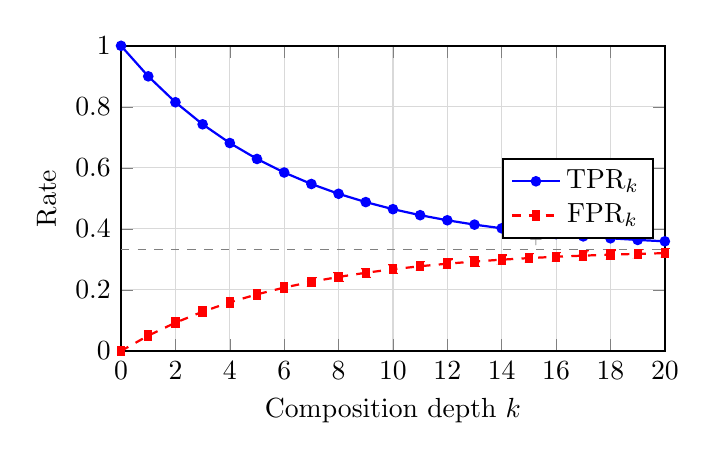
\begin{tikzpicture}
\begin{axis}[
	width=0.7\textwidth,
	height=0.45\textwidth,
	xlabel={Composition depth $k$},
	ylabel={Rate},
	xmin=0, xmax=20,
	ymin=0, ymax=1,
	legend style={at={(0.98,0.5)}, anchor=east},
	ymajorgrids, xmajorgrids,
	major grid style={gray!30},
	thick,
	xtick={0,2,...,20},
]
\addplot[blue, solid, mark=*, mark size=1.5pt] coordinates {
	(0,1.00000000) (1,0.90000000) (2,0.81500000)
	(3,0.74275000) (4,0.68133750) (5,0.62913688)
	(6,0.58476634) (7,0.54705139) (8,0.51499368)
	(9,0.48774463) (10,0.46458294) (11,0.44489550)
	(12,0.42816117) (13,0.41393700) (14,0.40184645)
	(15,0.39156948) (16,0.38283406) (17,0.37540895)
	(18,0.36909761) (19,0.36373297) (20,0.35917302)
};
\addlegendentry{TPR$_k$}
\addplot[red, dashed, mark=square*, mark size=1.5pt] coordinates {
	(0,0.00000000) (1,0.05000000) (2,0.09250000)
	(3,0.12862500) (4,0.15933125) (5,0.18543156)
	(6,0.20761683) (7,0.22647430) (8,0.24250316)
	(9,0.25612768) (10,0.26770853) (11,0.27755225)
	(12,0.28591941) (13,0.29303150) (14,0.29907678)
	(15,0.30421526) (16,0.30858297) (17,0.31229553)
	(18,0.31545120) (19,0.31813352) (20,0.32041349)
};
\addlegendentry{FPR$_k$}
\addplot[gray, thin, dashed, forget plot, domain=0:20] {1/3};
\node[anchor=west, gray] at (axis cs:14.5,0.37) {$\scriptstyle\frac{\fprate}{\fprate+\fnrate}$};
\end{axis}
\end{tikzpicture}
\caption{True positive rate and false positive rate under $k$-fold
composition of the approximate identity
$\APFun{id}[\fprate][\tprate]$ with $\fprate = 0.05$ and $\tprate = 0.90$.
Both rates converge to the stationary point
$\fprate/(\fprate + \fnrate) = 1/3$, where $\fnrate = 1 - \tprate$.
At high $k$, the approximation degrades toward a coin flip weighted by the
channel's stationary distribution.}
\label{fig:kfold_composition}
\end{figure}

In an \emph{algebra of sets} $(\PS{\Set{U}}, \SetIntersection, \SetUnion, \SetComplement, \Set{U}, \EmptySet)$, we may compose sets to form new sets.
When these sets model \emph{random approximate sets}, then their compositions model \emph{higher-order} random approximate sets, e.g.,
$\SetUnion[\ASet{A}[\fprate_1][\tprate_1]][\ASet{B}[\fprate_2][\tprate_2]]$
models a higher-order random approximate set which does not obey the second-order model; rather, it partitions the negative set such that each partition may have a different false positive rate and similarly for the positive set.

This contrasts with $\AT{\left(\SetUnion[\Set{A}][\Set{B}]\right)}[\fprate][\tprate]$, in which the false positive rate for the negative elements are uniformly distributed and likewise for the positive elements.
We call these random approximate sets \emph{second-order} approximations.
For completeness, the \emph{zeroth-order} are the objective sets, e.g., the zeroth-order approximation of $\SetUnion[\Set{A}][\Set{B}]$ is $\SetUnion[\Set{A}][\Set{B}]$.
The complexity of the probabilistic model increases as the order increases.

\subsection{Probability space}
\label{sec:prob_model}
The sample space is $\Omega = 2^U$, and the probability space is $(\Omega, \PS{\Omega}, P)$.
By \cref{asm:element_indep}, the conditional distribution of $\tilde{A}$ given the objective set $A$ factorizes element-wise:
\begin{equation}
    \Prob{\tilde{A} = S \Given A} = \prod_{x \in U} \Prob{\mathbf{1}_{\tilde{A}}(x) = \mathbf{1}_S(x) \Given \mathbf{1}_A(x)},
\end{equation}
where each factor equals $\tprate$ or $\fprate$ (if the element tests positive) or $\fnrate$ or $\tnrate$ (if it tests negative), depending on whether $x \in A$.

\begin{remark}[Latent and observed sets]
\label{rem:latent_observed}
The Bernoulli set model induces a duality between the \emph{latent} (objective) set $A$
and the \emph{observed} (approximate) set $\tilde{A}$.
Given the error model, the observed set constrains the possible latent sets.
For instance, if $\tilde{A}$ is a positive approximate set ($\fnrate = 0$),
then $A \subseteq \tilde{A}$: every element of $\tilde{A}$ is either a true positive
or a false positive, so the latent set must be a subset of the observed set.
Conversely, elements absent from $\tilde{A}$ are certainly absent from $A$.
\end{remark}


Consider the following example.
\begin{example}[Boolean universe]
\label{ex:boolean_universe}
	Let the universal set be $U = \{\top, \bot\}$ (the Boolean values \emph{true} and \emph{false}) and let the objective set be $A = \{\top\}$.
	A Bernoulli set $\tilde{A}^\fprate_\tprate$ over this universe has four possible outcomes, enumerated by the probability mass function
	\begin{equation}
	p_{\tilde{A}^\fprate_\tprate}(\Set{X}) =
	\begin{cases}
	\fnrate \cdot \tnrate & \Set{X} = \EmptySet,\\
	\fnrate \cdot \fprate & \Set{X} = \{\bot\},\\
	\tprate \cdot \tnrate & \Set{X} = \{\top\},\\
	\tprate \cdot \fprate & \Set{X} = \{\top, \bot\}.
	\end{cases}
	\end{equation}
	The outcome $\Set{X} = \{\top, \bot\}$ means both a true positive ($\top \in \tilde{A}$) and a false positive ($\bot \in \tilde{A}$) occurred.
	The outcome $\Set{X} = \{\bot\}$ means a false positive and a false negative occurred simultaneously.
	In the positive approximate set ($\fnrate = 0$), only $\Set{X} \in \{\{\top\}, \{\top, \bot\}\}$ are reachable, so $A \subseteq \tilde{A}$ with certainty.
\end{example}

\begin{remark}[Membership tests as Bernoulli Booleans]
\label{rem:membership_boolean}
For a Bernoulli set over an arbitrary universe $U$, the membership test $x \in \tilde{A}$ returns a Boolean value that is itself a Bernoulli approximation of the latent answer $x \in A$.
Consider a positive approximate set such as a Bloom filter, where $\fnrate = 0$.
If we query an element $x$ and observe $x \in \tilde{A}_+$, the result may be a false positive: $x$ might not belong to the latent set $A$.
If we observe $x \notin \tilde{A}_+$, the result is certainly a true negative: $x \notin A$.
Thus each membership query projects the set-level Bernoulli model onto the Boolean universe of \cref{ex:boolean_universe}, yielding a single Bernoulli Boolean whose error structure is inherited from the underlying set.
This pattern extends beyond data structures.
The Miller--Rabin primality test returns ``composite'' (certainly correct) or ``probably prime'' (false positive with probability at most $1/4$ per round), making its output a positive Bernoulli Boolean: the latent answer is $\{\text{prime}\}$ or $\{\text{composite}\}$, and the observed answer is a one-sided approximation with $\fnrate = 0$ and $\fprate \leq 1/4$.
More generally, any randomized decision procedure with one-sided error produces Bernoulli Booleans.
\end{remark}

%%%%%%%%%%%%%%%%%%%%%%%%%%%%%%%%%

%%%%%%%%%%%%%%%%%%%%%%%%%%%%%%%%%
% Distributions of error counts
%%%%%%%%%%%%%%%%%%%%%%%%%%%%%%%%%%%
\section{Distributions of error counts}
\label{sec:characteristics}
The error rate on some identically distributed subset is an \emph{expectation}.
However, some \emph{error measures} span multiple subsets, such as positives and negatives.
Any such error measure may be modeled as a \emph{Bernoulli mixture}.

We are typically interested in the error rates of \emph{special} subsets.
For example, if we have a universal set $\Set{X}$ and with probability $P(x)$ an element $x \in \Set{X}$ is tested for membership in a collection of sets over $\Set{X}$, then to reduce the expected error rate on membership tests elements with higher probability of being tested should be assigned smaller error rates.


The second-order random approximate sets are \emph{parameterized} by the \emph{expected} rates of two types of error, false negative and false positive rates.
In this section, we derive the distribution for these rates.

\begin{definition}
The uncertain number of \emph{negatives} is a random variable denoted by $\RV{N}$ and is statistically dependent on $R$,
\begin{equation}
\RV{N} = |\RV{R}^c|,
\end{equation}
\end{definition}

\begin{definition}
The uncertain number of false positives is a random variable denoted by $\FP$ and is statistically dependent on $\RV{N}$ and $\alpha$,
\begin{equation}
	\FP = \RV{N} \alpha.
\end{equation}
\end{definition}

The number of false positives given a specific number of negatives is given by the following theorem.
\begin{theorem}
\label{thm:fpbinom}
The random number of false positives $\FP$ given $\RV{N} = n$ in the second-order random approximate set $\tilde{\RV{R}}[\fprate]$ is given by
\begin{equation}
	\FP_n = n \alpha
\end{equation}
with a distribution given by
\begin{equation}
    \FP_n \sim \bindist(n, \fprate).
\end{equation}
\end{theorem}
\begin{proof}
By \cref{prop:element_rates}, the uncertain outcome that a negative element \emph{tests} as positive is a Bernoulli trial with a mean $\fprate$.
Since there are $n$ such independent and identically distributed trials, the number of false positives is binomially distributed with a mean $n \fprate$.
\end{proof}

The false positive rate $\fprate$ is an \emph{expectation}.
However, the false positive rate of a realization of a random approximate set $\tilde{S}[\fprate]$ is \emph{uncertain}.
\begin{theorem}
\label{thm:fpr}
The random false positive rate $\alpha$ conditioned on $\RV{N} = n$ is denoted by $\alpha_n$ and has a distribution given by
\begin{equation}
    \alpha_n = \frac{\FP_n}{n},
\end{equation}
with an expectation $\fprate$, variance $\fprate(1-\fprate) / n$, and probability mass function
\begin{equation}
	p_{\alpha_n}(\fprateob | \fprate) = p_{\FP_n}(\fprateob n | \fprate)
\end{equation}
over the support $\SetBuilder{ \frac{j}{n} \in \RatSet}{j \in \{0,\ldots,n\}}$.
\end{theorem}
\begin{proof}
By \cref{def:fprate}, the false positive rate is given by the ratio of the number of false positives to the total number of negatives.
By \cref{thm:fpbinom}, given that there are $n$ negatives, the number of false positives is a random variable denoted by $\FP_n$.
Therefore, the false positive rate, as a function of $\FP_n$, is the random variable $\frac{\FP_n}{n}$.
The \emph{expected} false positive rate is
\begin{equation}
    \Expect{\frac{\FP_n}{n}} = \frac{1}{n}\Expect{\FP_n} = \fprate
\end{equation}
and its variance is
\begin{equation}
    \Var{\frac{\FP_n}{n}} = \frac{1}{n^2}\Var{\FP_n} = \frac{\fprate(1-\fprate)}{n}.
\end{equation}
Finally, $\alpha_n = \FP_n / n$ is a \emph{scaled} transformation of the binomial distribution.
Thus, since $\FP_n = n \alpha_n$,
\begin{equation}
	p_{\alpha_n}(\fprateob_n | \fprate) = p_{\FP_n}(n \fprateob).
\end{equation}
\end{proof}
The following corollary immediately follows.
\begin{corollary}
	\label{cor:tnbinom}
	Given $n$ negatives, the number of \emph{true negatives} in a random approximate set with a false positive rate $\fprate$ is a random variable denoted by $\TN_n$ with a distribution given by
	\begin{equation}
	\TN_n = n - \FP_n \sim \bindist\!\left(n, 1-\fprate\right).
	\end{equation}
	By definition, the \emph{true negative rate} $\mathrm{TNR}_n = \TN_n / n = 1 - \alpha_n$.
\end{corollary}

By \cref{thm:fpr}, the more negatives there are, the lower the variance.
\begin{corollary}
\label{cor:fpr_as_vareps}
	Given \emph{countably infinite} negatives, a random approximate set with a false positive rate $\fprate$ is \emph{certain} to obtain $\fprate$.
\end{corollary}
\begin{proof}
We know that the \emph{expected} value for each of the random variables in this sequence is $\fprate$ and the variance is $\fprate(1-\fprate)/n$.
Immediately, we see that as $n$ increases, the distribution of false positives must become more concentrated around $\fprate$.
As $n \to \infty$, the variance goes to $0$, i.e., the distribution becomes degenerate with all of the probability mass assigned to the mean. See \cref{app:cor_fpr_as_vareps} for a more rigorous proof.
\end{proof}

The fewer negatives, the greater the variance.
The maximum possible variance, when $n=1$ and $\fprate = 0.5$, is $0.25$, may be used as the most \emph{pessimistic} estimate given a situation where we have no information about the false positive rate $\fprate$ and the cardinality of the universal set.

A degenerate case is given by letting $n = 0$, corresponding to a random approximate set of the universal set which has no negative elements that can be tested.
Respectively, only random \emph{negative} or \emph{positive} approximate sets may be generated for the universal set or empty set.

The number of false negatives is given by the following theorem.
\begin{theorem}
\label{thm:fnbinom}
Given $p$ positives, the uncertain number of \emph{false negatives} in random approximate sets with a false negative rate $\fnrate$ is modeled as a binomial distributed random variable denoted by $\FN_p$,
\begin{equation}
	\FN_p \sim \bindist(p, \fnrate).
\end{equation}
\end{theorem}
\begin{proof}
By \cref{prop:element_rates}, the probability that a positive element \emph{tests} as negative is $\fnrate$.
Thus, each test is a Bernoulli trial.
Since there are $p = \Card{\Set{S}}$ such independent and identically distributed trials with a probability of ``success'' $\fnrate$, the number of false negatives is binomially distributed.
\end{proof}

The false negative rate $\fnrate$ is an \emph{expectation}.
However, the false negative rate of an approximate set $\tilde{S}$ parameterized by $\fnrate$ is \emph{uncertain}.
\begin{theorem}
\label{thm:fnr}
The false negative rate realizes an uncertain value as given by
\begin{equation}
    \beta_p = \frac{\FN_p}{p}
\end{equation}
with a support $\SetBuilder{j / p}{j = 0,\ldots,p}$, an expectation
$\fnrate$, and a variance $\fnrate(1-\fnrate) / p$.
\end{theorem}
The proof follows the same logic as the proof for \cref{thm:fpr}, with $\FN_p \sim \bindist(p, \fnrate)$ in place of $\FP_n \sim \bindist(n, \fprate)$.

In the companion paper~\cite{bernoulliComposition}, we consider set-theoretic
operations like \emph{complements}. The \emph{complement} operator applied to an
approximate set of a set with countably infinite negatives is an approximate set
of a set with countably infinite positives.
\begin{corollary}
An approximate set of a set with countably infinite positives has a false
negative rate that is \emph{certain} to obtain $\fnrate$.
\end{corollary}
The proof follows the same logic as the proof for \cref{cor:fpr_as_vareps}, replacing negatives with positives and $\fprate$ with $\fnrate$.

The number of true positives is given by the following corollary.
\begin{corollary}
\label{cor:tpbinom}
Given $p$ positives, the number of \emph{true positives} in an approximate set
with a false negative rate $\fnrate$ is a random variable denoted by $\TP_p$
with a distribution given by
\begin{equation}
    \TP_p \sim \bindist(p, \tprate).
\end{equation}
By definition, the \emph{true positive rate} is given by $\TPR_p = 1 -
\beta_p$.
\end{corollary}
The proof follows the same logic as the proof for \cref{thm:fpr}, with $\TP_p = p - \FN_p$ and $\tprate = 1 - \fnrate$.

Many other properties of random approximate sets follow from these distributions.
For instance, the distribution of $\Card{\tilde{A}^\fprate_\tprate}$ given $p$ positives is
\begin{equation}
	\Card{\tilde{A}^\fprate_\tprate} = \TP_p + \FP_{u - p}
\end{equation}
where $u$ is the cardinality of the universal set. This sum has an expectation of $(u - p) \fprate + p \tprate$ and variance of $(u - p) \fprate(1-\fprate) + p \tprate(1-\tprate)$, which is the generalization of the binomial distribution known as the \emph{Poisson binomial distribution}.

If we do not know the number of positives $p$, the cardinality $\Set{A}$, but have observed $\tilde{A}^\fprate_\tprate = \Set{B}$, then $\Set{B}$ has a cardinality that tends to be centered around $u \fprate + p (\tprate - \fprate)$.
Solving for $p$ yields a method of moments estimator
\begin{equation}
	\widehat{p} = \frac{|\Set{B}| - u \fprate}{\tprate - \fprate}.
\end{equation}
If the universal set $U$ is infinite, then this estimator is undefined.

\subsection{Asymptotic limits}
\label{sec:asymtotic}
The false positive and false negative rates are a function of the cardinality of the objective and universal sets.
The limiting distributions for the false positive and true positive rates are given by the following theorems.
\begin{theorem}
    \label{thm:approxfpr}
    By \cref{thm:fpr}, the uncertain false positive rate $\alpha_n$ converges in
    distribution to the normal distribution with a mean $\fprate$ and a
    variance $\fprate(1-\fprate)/n$, written
    \begin{equation}
    \label{eq:approxfpr}
	    \alpha_n \xrightarrow{d} \normdist(\fprate, \fprate(1-\fprate) / n).
    \end{equation}
    Similarly, by \cref{cor:tpbinom}, the uncertain true positive rate of an approximate  set of $p$ positives, denoted by $\TPR_p$, converges in distribution to the normal distribution with a mean $\tprate$ and a variance $\tprate(1-\tprate)/p$, written
    \begin{equation}
    \label{eq:approxtpr}
    	\TPR_p \xrightarrow{d} \normdist(\tprate, \tprate(1-\tprate) / p).
    \end{equation}
\end{theorem}
\begin{proof}
    By \cref{thm:fpr}, given $n$ negatives, the false positive rate is
    \begin{equation}
    	\alpha_n = \frac{\RV{X_1}}{n} + \cdots + \frac{\RV{X_n}}{n},
    \end{equation}
    where $\RV{X_1},\ldots,\RV{X_n}$ are $n$ independent Bernoulli trials each with a mean $\fprate$ and a variance $\fprate(1-\fprate)$.
    Therefore, by the central limit theorem~\cite{feller2}, $\alpha_n$ converges in distribution to a normal distribution with a mean $\fprate$  and a variance $\fprate(1-\fprate)/n$.
    The proof for the true positive rate follows the same logic, replacing $\fprate$ with $\tprate$, $n$ with $p$, and negatives with positives.
\end{proof}
By \cref{eq:approxfpr,eq:approxtpr},
\begin{equation}
	\mathrm{TNR}_n \xrightarrow{d} \normdist\!\left(1-\fprate, \fprate(1-\fprate) / n\right) \text{ and } \beta_p \xrightarrow{d} \normdist\!\left(1-\tprate, \tprate(1-\tprate) / p\right).
\end{equation}

The Bernoulli set model is the \emph{maximum entropy} distribution over $\{0,1\}^u$ subject to the constraint that each element has a fixed marginal error probability: the binomial distribution maximizes entropy over $\{0,\ldots,n\}$ for a given mean~\cite{coverThomas}.
As a consequence, any $\gamma$-confidence intervals derived from this model are the widest possible for the indicated $\gamma$ and therefore represent a worst-case uncertainty.

If we generate an approximate set, the uncertain false positive and true positive rates realize certain values, i.e., $\alpha_n = \fprateob$ and $\TPR_p = \tprateob$.
If the sample space is countably infinite, the distribution is degenerate, e.g., $\alpha_n = \fprate$ with probability $1$.
However, for finite sample spaces, the outcomes are uncertain.
If these outcomes can be \emph{observed}, e.g., it is not too costly to compute, the exact values $\fprateob$ and $\tprateob$ may be recorded.
If these outcomes cannot be observed, e.g., it is too costly to compute or the information to compute $\fprateob$ or $\tprateob$ is not available, we may use the probabilistic model to inform us about the distribution of false positive rates.

\emph{Confidence intervals} that contain the true false positive rate $\fprateob$ and the true true positive rate $\tprateob$ are given by the following theorem.
\begin{theorem}
    Given a random approximate set parameterized by $\fprate$ and $\tprate$, asymptotic $\gamma \cdot 100\%$ confidence intervals for the false positive rate and true positive rate are respectively
    \begin{equation}
    \label{eq:conf_fpr}
    \fprate \pm \sqrt{\frac{\fprate(1-\fprate)}{n}} \Phi^{-1}\!\left(\frac{1+\gamma}{2}\right)
    \end{equation}
    and
    \begin{equation}
    \label{eq:conf_tpr}
    \tprate \pm \sqrt{\frac{\tprate(1-\tprate)}{p}} \Phi^{-1}\!\left(\frac{1+\gamma}{2}\right),
    \end{equation}
    where $\Phi^{-1} : [0,1] \to \RealSet$ is the inverse cumulative distribution function of the standard normal.
\end{theorem}
\begin{proof}
By \cref{thm:approxfpr}, $\alpha_n$ is asymptotically normal with mean $\fprate$ and variance $\sigma^2 = \fprate(1-\fprate)/n$.
Standardizing, $Z = (\alpha_n - \fprate)/\sigma \xrightarrow{d} \normdist(0,1)$.
A $\gamma$-level confidence interval requires
$\Prob{-z_\gamma \leq Z \leq z_\gamma} = \gamma$,
where $z_\gamma = \Phi^{-1}\!\left(\frac{1+\gamma}{2}\right)$.
Substituting and solving for $\alpha_n$ yields
$\fprate \pm \sigma \, z_\gamma = \fprate \pm \sqrt{\fprate(1-\fprate)/n}\;\Phi^{-1}\!\left(\frac{1+\gamma}{2}\right)$.
The argument for the true positive rate is identical with $\tprate$ and $p$ replacing $\fprate$ and $n$.
\end{proof}
As a worst-case (maximum uncertainty), we may let $n = p = 1$ in \cref{eq:conf_fpr,eq:conf_tpr}.
%However, if the universe is large and the objective sets are relatively small, a slightly optimistic confidence interval for $\fprate$ is provided by letting $n = \Card{\Set{U}}$.

%%%%%%%%%%%%%%%%%%%%%%%%%%%%%%%%%
% Set-theoretic operations on Bernoulli sets
%%%%%%%%%%%%%%%%%%%%%%%%%%%%%%%%%

\section{Set-theoretic operations}
\label{sec:set_theory}
In this section, we derive the error rates of Bernoulli sets under the
standard set-theoretic operations: complement, union, intersection, and set
difference.
Throughout, we assume that the Bernoulli sets $\tilde{A}_1$ and
$\tilde{A}_2$ approximate objective sets $A_1$ and $A_2$ respectively over
a common finite universal set $U$ with cardinality $u = |U|$.
The Bernoulli set $\tilde{A}_i$ has false positive rate $\fprate_i$ and
false negative rate $\fnrate_i$ for $i \in \{1,2\}$.
By the axioms of the Bernoulli set model, the membership errors of distinct
elements are independent.

\begin{assumption}[Cross-set independence]
\label{asm:cross_set_indep}
The Bernoulli sets $\tilde{A}_1$ and $\tilde{A}_2$ are constructed using independent randomness: for all $x \in U$, the error indicators $\mathbf{1}_{\tilde{A}_1}(x) \neq \mathbf{1}_{A_1}(x)$ and $\mathbf{1}_{\tilde{A}_2}(x) \neq \mathbf{1}_{A_2}(x)$ are independent.
\end{assumption}

\subsection{Complement}
\label{sec:complement}
The complement operation exchanges the roles of positives and negatives.
Accordingly, false positives become false negatives and vice versa.

\begin{theorem}[Complement error rates]
\label{thm:complement_rates}
Let $\tilde{A}$ be a Bernoulli set approximating $A$ with false positive
rate $\fprate$ and false negative rate $\fnrate$.
Then the complement $\SetComplement[\tilde{A}]$ is a Bernoulli set
approximating $A^c$ with false positive rate $\fnrate$ and false negative
rate $\fprate$.
\end{theorem}
\begin{proof}
The positives of $A^c$ are exactly the negatives of $A$, and the negatives
of $A^c$ are exactly the positives of $A$.

A false positive of $\SetComplement[\tilde{A}]$ with respect to $A^c$
occurs when an element $x \notin A^c$ (i.e., $x \in A$) satisfies
$x \in \SetComplement[\tilde{A}]$, which holds if and only if
$x \notin \tilde{A}$.
Since $x \in A$, the event $x \notin \tilde{A}$ is a false negative of
$\tilde{A}$, which occurs with probability $\fnrate$.
Therefore the false positive rate of $\SetComplement[\tilde{A}]$ with
respect to $A^c$ is $\fnrate$.

A false negative of $\SetComplement[\tilde{A}]$ with respect to $A^c$
occurs when an element $x \in A^c$ (i.e., $x \notin A$) satisfies
$x \notin \SetComplement[\tilde{A}]$, which holds if and only if
$x \in \tilde{A}$.
Since $x \notin A$, the event $x \in \tilde{A}$ is a false positive of
$\tilde{A}$, which occurs with probability $\fprate$.
Therefore the false negative rate of $\SetComplement[\tilde{A}]$ with
respect to $A^c$ is $\fprate$.
\end{proof}

\begin{remark}
\Cref{thm:complement_rates} establishes that complementation maps positive
Bernoulli sets ($\fnrate = 0$) to negative Bernoulli sets ($\fprate = 0$)
and vice versa.
\end{remark}

\subsection{Union}
\label{sec:union}
We derive the false positive and false negative rates of the union
$\tilde{A}_1 \cup \tilde{A}_2$ as a Bernoulli set approximating
$A_1 \cup A_2$.

\begin{theorem}[Union false positive rate]
\label{thm:union_fprate}
The union $\tilde{A}_1 \cup \tilde{A}_2$ has false positive rate
\begin{equation}
\label{eq:union_fpr}
\fprate = 1 - (1 - \fprate_1)(1 - \fprate_2)
\end{equation}
with respect to $A_1 \cup A_2$.
\end{theorem}
\begin{proof}
Let $x \notin A_1 \cup A_2$.
Then $x \notin A_1$ and $x \notin A_2$, so $x$ is a negative of both
$A_1$ and $A_2$.
A false positive of the union occurs when
$x \in \tilde{A}_1 \cup \tilde{A}_2$, i.e., when
$x \in \tilde{A}_1$ or $x \in \tilde{A}_2$ (or both).
By the independence of errors across the two Bernoulli sets (\cref{asm:cross_set_indep}),
\begin{align}
\Prob{x \in \tilde{A}_1 \cup \tilde{A}_2 \Given x \notin A_1 \cup A_2}
&= 1 - \Prob{x \notin \tilde{A}_1 \cup \tilde{A}_2
    \Given x \notin A_1 \cup A_2} \\
&= 1 - \Prob{x \notin \tilde{A}_1 \Given x \notin A_1}\,
       \Prob{x \notin \tilde{A}_2 \Given x \notin A_2} \\
&= 1 - (1 - \fprate_1)(1 - \fprate_2).
\end{align}
Since this probability is the same for every negative of $A_1 \cup A_2$,
the false positive rate of the union is
$\fprate = 1 - (1 - \fprate_1)(1 - \fprate_2)$.
\end{proof}

\begin{theorem}[Union false negative rate]
\label{thm:union_fnrate}
The union $\tilde{A}_1 \cup \tilde{A}_2$ has false negative rate
\begin{equation}
\label{eq:union_fnr}
\fnrate = w_1 \fnrate_1 (1 - \fprate_2)
        + w_2 \fnrate_2 (1 - \fprate_1)
        + w_3 \fnrate_1 \fnrate_2
\end{equation}
with respect to $A_1 \cup A_2$, where
\begin{equation}
\label{eq:union_weights}
w_1 = \frac{|A_1 \setminus A_2|}{|A_1 \cup A_2|}, \quad
w_2 = \frac{|A_2 \setminus A_1|}{|A_1 \cup A_2|}, \quad
w_3 = \frac{|A_1 \cap A_2|}{|A_1 \cup A_2|}.
\end{equation}
\end{theorem}
\begin{proof}
A false negative of the union occurs when an element $x \in A_1 \cup A_2$
satisfies $x \notin \tilde{A}_1 \cup \tilde{A}_2$, i.e.,
$x \notin \tilde{A}_1$ and $x \notin \tilde{A}_2$.
We partition the positives $A_1 \cup A_2$ into three disjoint regions:
\begin{enumerate}[label=(\roman*)]
    \item $A_1 \setminus A_2$: elements in $A_1$ only,
    \item $A_2 \setminus A_1$: elements in $A_2$ only,
    \item $A_1 \cap A_2$: elements in both $A_1$ and $A_2$.
\end{enumerate}

For region~(i), let $x \in A_1 \setminus A_2$.
Then $x \in A_1$ and $x \notin A_2$.
By independence,
\begin{equation}
\Prob{x \notin \tilde{A}_1 \text{ and } x \notin \tilde{A}_2
    \Given x \in A_1,\, x \notin A_2}
= \fnrate_1 (1 - \fprate_2).
\end{equation}

For region~(ii), let $x \in A_2 \setminus A_1$.
Then $x \notin A_1$ and $x \in A_2$.
By independence,
\begin{equation}
\Prob{x \notin \tilde{A}_1 \text{ and } x \notin \tilde{A}_2
    \Given x \notin A_1,\, x \in A_2}
= (1 - \fprate_1) \fnrate_2.
\end{equation}

For region~(iii), let $x \in A_1 \cap A_2$.
Then $x \in A_1$ and $x \in A_2$.
By independence,
\begin{equation}
\Prob{x \notin \tilde{A}_1 \text{ and } x \notin \tilde{A}_2
    \Given x \in A_1,\, x \in A_2}
= \fnrate_1 \fnrate_2.
\end{equation}

By the law of total probability, weighting each region by its proportion
of $|A_1 \cup A_2|$,
\begin{equation}
\fnrate
= w_1 \fnrate_1 (1 - \fprate_2)
+ w_2 \fnrate_2 (1 - \fprate_1)
+ w_3 \fnrate_1 \fnrate_2,
\end{equation}
where $w_1$, $w_2$, and $w_3$ are as defined in
\cref{eq:union_weights}.
\end{proof}

\begin{corollary}[Union of positive Bernoulli sets]
\label{cor:union_positive}
If $\tilde{A}_1$ and $\tilde{A}_2$ are positive Bernoulli sets
($\fnrate_1 = \fnrate_2 = 0$), then $\tilde{A}_1 \cup \tilde{A}_2$ is a
positive Bernoulli set with
\begin{equation}
\fprate = \fprate_1 + \fprate_2 - \fprate_1 \fprate_2
\quad \text{and} \quad
\fnrate = 0.
\end{equation}
\end{corollary}

\begin{corollary}[Union of negative Bernoulli sets]
\label{cor:union_negative}
If $\tilde{A}_1$ and $\tilde{A}_2$ are negative Bernoulli sets
($\fprate_1 = \fprate_2 = 0$), then $\tilde{A}_1 \cup \tilde{A}_2$ is a
negative Bernoulli set with
\begin{equation}
\fprate = 0
\quad \text{and} \quad
\fnrate = w_1 \fnrate_1 + w_2 \fnrate_2
        + w_3 \fnrate_1 \fnrate_2,
\end{equation}
where $w_1$, $w_2$, $w_3$ are as in \cref{eq:union_weights}.
\end{corollary}

\subsection{Intersection}
\label{sec:intersection}
We now derive the error rates of the intersection
$\tilde{A}_1 \cap \tilde{A}_2$ as a Bernoulli set approximating
$A_1 \cap A_2$.

\begin{theorem}[Intersection false negative rate]
\label{thm:intersect_fnrate}
The intersection $\tilde{A}_1 \cap \tilde{A}_2$ has false negative rate
\begin{equation}
\label{eq:intersect_fnr}
\fnrate = 1 - (1 - \fnrate_1)(1 - \fnrate_2)
\end{equation}
with respect to $A_1 \cap A_2$.
\end{theorem}
\begin{proof}
Let $x \in A_1 \cap A_2$.
Then $x \in A_1$ and $x \in A_2$.
A false negative of the intersection occurs when
$x \notin \tilde{A}_1 \cap \tilde{A}_2$, i.e., when
$x \notin \tilde{A}_1$ or $x \notin \tilde{A}_2$ (or both).
By the independence of errors,
\begin{align}
\Prob{x \notin \tilde{A}_1 \cap \tilde{A}_2
    \Given x \in A_1 \cap A_2}
&= 1 - \Prob{x \in \tilde{A}_1 \cap \tilde{A}_2
    \Given x \in A_1 \cap A_2} \\
&= 1 - \Prob{x \in \tilde{A}_1 \Given x \in A_1}\,
       \Prob{x \in \tilde{A}_2 \Given x \in A_2} \\
&= 1 - (1 - \fnrate_1)(1 - \fnrate_2).
\end{align}
Since this probability is the same for every positive of $A_1 \cap A_2$,
the false negative rate is $\fnrate = 1 - (1 - \fnrate_1)(1 - \fnrate_2)$.
\end{proof}

\begin{theorem}[Intersection false positive rate]
\label{thm:intersect_fprate}
The intersection $\tilde{A}_1 \cap \tilde{A}_2$ has false positive rate
\begin{equation}
\label{eq:intersect_fpr}
\fprate = w_1 (1 - \fnrate_1) \fprate_2
        + w_2 \fprate_1 (1 - \fnrate_2)
        + w_3 \fprate_1 \fprate_2
\end{equation}
with respect to $A_1 \cap A_2$, where
\begin{equation}
\label{eq:intersect_weights}
w_1 = \frac{|A_1 \setminus A_2|}{u - |A_1 \cap A_2|}, \quad
w_2 = \frac{|A_2 \setminus A_1|}{u - |A_1 \cap A_2|}, \quad
w_3 = \frac{|U \setminus (A_1 \cup A_2)|}{u - |A_1 \cap A_2|}.
\end{equation}
\end{theorem}
\begin{proof}
A false positive of the intersection occurs when an element
$x \notin A_1 \cap A_2$ satisfies $x \in \tilde{A}_1 \cap \tilde{A}_2$,
i.e., $x \in \tilde{A}_1$ and $x \in \tilde{A}_2$.
We partition the negatives of $A_1 \cap A_2$
(the set $U \setminus (A_1 \cap A_2)$) into three disjoint regions:
\begin{enumerate}[label=(\roman*)]
    \item $A_1 \setminus A_2$: elements in $A_1$ but not $A_2$,
    \item $A_2 \setminus A_1$: elements in $A_2$ but not $A_1$,
    \item $U \setminus (A_1 \cup A_2)$: elements in neither
        $A_1$ nor $A_2$.
\end{enumerate}

For region~(i), let $x \in A_1 \setminus A_2$.
Then $x \in A_1$ and $x \notin A_2$.
By independence,
\begin{equation}
\Prob{x \in \tilde{A}_1 \text{ and } x \in \tilde{A}_2
    \Given x \in A_1,\, x \notin A_2}
= (1 - \fnrate_1)\, \fprate_2.
\end{equation}

For region~(ii), let $x \in A_2 \setminus A_1$.
Then $x \notin A_1$ and $x \in A_2$.
By independence,
\begin{equation}
\Prob{x \in \tilde{A}_1 \text{ and } x \in \tilde{A}_2
    \Given x \notin A_1,\, x \in A_2}
= \fprate_1\, (1 - \fnrate_2).
\end{equation}

For region~(iii), let $x \in U \setminus (A_1 \cup A_2)$.
Then $x \notin A_1$ and $x \notin A_2$.
By independence,
\begin{equation}
\Prob{x \in \tilde{A}_1 \text{ and } x \in \tilde{A}_2
    \Given x \notin A_1,\, x \notin A_2}
= \fprate_1\, \fprate_2.
\end{equation}

By the law of total probability, weighting by the proportion of
$|U \setminus (A_1 \cap A_2)|$ contributed by each region,
\begin{equation}
\fprate
= w_1 (1 - \fnrate_1) \fprate_2
+ w_2 \fprate_1 (1 - \fnrate_2)
+ w_3 \fprate_1 \fprate_2,
\end{equation}
where $w_1$, $w_2$, $w_3$ are as in
\cref{eq:intersect_weights}.
\end{proof}

\begin{corollary}[Intersection of positive Bernoulli sets]
\label{cor:intersect_positive}
If $\tilde{A}_1$ and $\tilde{A}_2$ are positive Bernoulli sets
($\fnrate_1 = \fnrate_2 = 0$), then $\tilde{A}_1 \cap \tilde{A}_2$ is a
positive Bernoulli set with
\begin{equation}
\fprate = w_1 \fprate_2 + w_2 \fprate_1
        + w_3 \fprate_1 \fprate_2
\quad \text{and} \quad
\fnrate = 0,
\end{equation}
where $w_1$, $w_2$, $w_3$ are as in
\cref{eq:intersect_weights}.
\end{corollary}

\begin{corollary}[Intersection of negative Bernoulli sets]
\label{cor:intersect_negative}
If $\tilde{A}_1$ and $\tilde{A}_2$ are negative Bernoulli sets
($\fprate_1 = \fprate_2 = 0$), then $\tilde{A}_1 \cap \tilde{A}_2$ is a
negative Bernoulli set with
\begin{equation}
\fprate = 0
\quad \text{and} \quad
\fnrate = \fnrate_1 + \fnrate_2 - \fnrate_1 \fnrate_2.
\end{equation}
\end{corollary}

\subsection{Set difference}
\label{sec:setdiff}
The set difference $A_1 \setminus A_2 = A_1 \cap A_2^c$ may be treated as
an intersection of $\tilde{A}_1$ with $\SetComplement[\tilde{A}_2]$.
By \cref{thm:complement_rates}, $\SetComplement[\tilde{A}_2]$ has false
positive rate $\fnrate_2$ and false negative rate $\fprate_2$ with respect
to $A_2^c$.
Substituting these rates into the intersection formulas yields the following
theorem.

\begin{theorem}[Set difference error rates]
\label{thm:setdiff_rates}
The set difference $\tilde{A}_1 \setminus \tilde{A}_2
= \tilde{A}_1 \cap \SetComplement[\tilde{A}_2]$ has error rates
\begin{align}
\label{eq:setdiff_fpr}
\fprate &= w_1 (1 - \fnrate_1)\, \fnrate_2
          + w_2 \fprate_1\, (1 - \fprate_2)
          + w_3 \fprate_1\, \fnrate_2, \\
\label{eq:setdiff_fnr}
\fnrate &= 1 - (1 - \fnrate_1)(1 - \fprate_2)
\end{align}
with respect to $A_1 \setminus A_2$, where
\begin{equation}
\label{eq:setdiff_weights}
w_1 = \frac{|A_1 \cap A_2|}{u - |A_1 \setminus A_2|}, \quad
w_2 = \frac{|U \setminus (A_1 \cup A_2)|}{u - |A_1 \setminus A_2|}, \quad
w_3 = \frac{|A_2 \setminus A_1|}{u - |A_1 \setminus A_2|}.
\end{equation}
\end{theorem}
\begin{proof}
Write $\tilde{A}_1 \setminus \tilde{A}_2
= \tilde{A}_1 \cap \SetComplement[\tilde{A}_2]$.
By \cref{thm:complement_rates}, $\SetComplement[\tilde{A}_2]$ approximates
$A_2^c$ with false positive rate $\fnrate_2$ and false negative rate
$\fprate_2$.
The objective set for the difference is
$A_1 \setminus A_2 = A_1 \cap A_2^c$.

For the false negative rate, apply \cref{thm:intersect_fnrate} to the
intersection of $\tilde{A}_1$ (FNR $\fnrate_1$) and
$\SetComplement[\tilde{A}_2]$ (FNR $\fprate_2$):
\begin{equation}
\fnrate = 1 - (1 - \fnrate_1)(1 - \fprate_2).
\end{equation}

For the false positive rate, we partition the negatives of
$A_1 \cap A_2^c$ (the set $U \setminus (A_1 \setminus A_2)$) into three
disjoint regions, mirroring the structure of \cref{thm:intersect_fprate}:
\begin{enumerate}[label=(\roman*)]
    \item $A_1 \cap A_2$: here $x \in A_1$ and $x \in A_2$, so
        $x \in \tilde{A}_1$ with probability $1 - \fnrate_1$ and
        $x \in \SetComplement[\tilde{A}_2]$ (i.e., $x \notin \tilde{A}_2$)
        with probability $\fnrate_2$.
        The contribution is $(1 - \fnrate_1)\,\fnrate_2$.

    \item $U \setminus (A_1 \cup A_2)$: here $x \notin A_1$ and
        $x \notin A_2$, so
        $x \in \tilde{A}_1$ with probability $\fprate_1$ and
        $x \in \SetComplement[\tilde{A}_2]$ with probability
        $1 - \fprate_2$.
        The contribution is $\fprate_1\,(1 - \fprate_2)$.

    \item $A_2 \setminus A_1$: here $x \notin A_1$ and $x \in A_2$, so
        $x \in \tilde{A}_1$ with probability $\fprate_1$ and
        $x \in \SetComplement[\tilde{A}_2]$ with probability $\fnrate_2$.
        The contribution is $\fprate_1\,\fnrate_2$.
\end{enumerate}

By the law of total probability, weighting by the proportions $w_1$,
$w_2$, and $w_3$ as defined in \cref{eq:setdiff_weights},
\begin{equation}
\fprate
= w_1 (1 - \fnrate_1)\, \fnrate_2
+ w_2 \fprate_1\, (1 - \fprate_2)
+ w_3 \fprate_1\, \fnrate_2. \qedhere
\end{equation}
\end{proof}

\begin{remark}
The false negative rate of the set difference
$\fnrate = 1 - (1 - \fnrate_1)(1 - \fprate_2)$ shows that even if
$\tilde{A}_1$ has no false negatives ($\fnrate_1 = 0$), a nonzero false
positive rate in $\tilde{A}_2$ induces false negatives in the difference,
since elements of $A_1 \setminus A_2$ that are false positives of
$\tilde{A}_2$ will be erroneously excluded.
\end{remark}

\subsection{Summary of error rates}
\label{sec:set_ops_summary}

\begin{table}[t]
\centering
\caption{Error rates of set-theoretic operations on Bernoulli sets.
The partition weights $w_1$, $w_2$, $w_3$ are operation-dependent;
see \cref{eq:union_weights,eq:intersect_weights,eq:setdiff_weights}
for their precise definitions.}
\label{tab:set_ops}
\begin{tabular}{@{} l l l @{}}
\toprule
\textbf{Operation}
    & \textbf{FPR} $\fprate$
    & \textbf{FNR} $\fnrate$ \\
\midrule
$\SetComplement[\tilde{A}_1]$
    & $\fnrate_1$
    & $\fprate_1$ \\[6pt]
$\tilde{A}_1 \cup \tilde{A}_2$
    & $1-(1-\fprate_1)(1-\fprate_2)$
    & $w_1\fnrate_1(1-\fprate_2)
      +w_2\fnrate_2(1-\fprate_1)
      +w_3\fnrate_1\fnrate_2$ \\[6pt]
$\tilde{A}_1 \cap \tilde{A}_2$
    & $w_1(1-\fnrate_1)\fprate_2
      +w_2\fprate_1(1-\fnrate_2)
      +w_3\fprate_1\fprate_2$
    & $1-(1-\fnrate_1)(1-\fnrate_2)$ \\[6pt]
$\tilde{A}_1 \setminus \tilde{A}_2$
    & $w_1(1-\fnrate_1)\fnrate_2
      +w_2\fprate_1(1-\fprate_2)
      +w_3\fprate_1\fnrate_2$
    & $1-(1-\fnrate_1)(1-\fprate_2)$ \\
\bottomrule
\end{tabular}
\end{table}

\Cref{tab:set_ops} summarizes the error rates derived in the preceding
subsections.

\begin{remark}[Unknown partition sizes]
\label{rem:unknown_partitions}
The partition weights $w_1, w_2, w_3$ require knowledge of the objective set cardinalities $|A_1|$, $|A_2|$, and $|A_1 \cap A_2|$, which are typically unknown in practice.
Three approaches handle this:
(a) if only upper bounds on $|A_i|$ are available, \cref{sec:intervals} provides interval-valued rates;
(b) worst-case bounds are obtained by optimizing the weights over the feasible region $w_1 + w_2 + w_3 = 1$, $w_i \geq 0$;
(c) the cardinalities may be estimated from the approximate sets themselves, e.g., $|\tilde{A}_1 \cap \tilde{A}_2|$ is a biased estimator of $|A_1 \cap A_2|$ with computable bias from the error rates.
\end{remark}

\begin{figure}[ht]
\centering
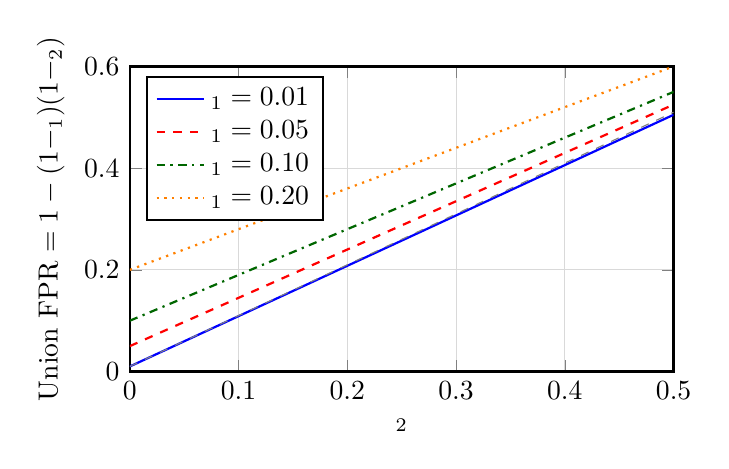
\begin{tikzpicture}
\begin{axis}[
	width=0.7\textwidth,
	height=0.45\textwidth,
	xlabel={$\fprate_2$},
	ylabel={Union FPR $= 1 - (1-\fprate_1)(1-\fprate_2)$},
	xmin=0, xmax=0.5,
	ymin=0, ymax=0.6,
	legend pos=north west,
	ymajorgrids, xmajorgrids,
	major grid style={gray!30},
	thick,
	samples=100,
	domain=0:0.5,
]
\addplot[blue, solid] {1-(1-0.01)*(1-x)};
\addlegendentry{$\fprate_1 = 0.01$}
\addplot[red, dashed] {1-(1-0.05)*(1-x)};
\addlegendentry{$\fprate_1 = 0.05$}
\addplot[black!60!green, dashdotted] {1-(1-0.10)*(1-x)};
\addlegendentry{$\fprate_1 = 0.10$}
\addplot[orange, dotted, thick] {1-(1-0.20)*(1-x)};
\addlegendentry{$\fprate_1 = 0.20$}
\addplot[gray, thin, dashed, forget plot] {x + 0.01};
\end{axis}
\end{tikzpicture}
\caption{Union false positive rate
$\fprate = 1 - (1-\fprate_1)(1-\fprate_2)$ as a function of $\fprate_2$
for several fixed values of $\fprate_1$.
The thin dashed gray line shows the additive approximation
$\fprate_1 + \fprate_2$ for $\fprate_1 = 0.01$;
for small rates, the union FPR is nearly additive, but the
product term $\fprate_1 \fprate_2$ becomes significant as rates grow.
By De Morgan duality, the intersection FNR has the same functional form
with $\fnrate_i$ replacing $\fprate_i$.}
\label{fig:union_fpr}
\end{figure}

\begin{example}[Numerical illustration of union error rates]
\label{ex:numerical_union}
Let $|U| = 1000$, $|A_1| = 100$, $|A_2| = 80$, and $|A_1 \cap A_2| = 30$.
Then $|A_1 \cup A_2| = 100 + 80 - 30 = 150$ and the partition weights for the union (\cref{eq:union_weights}) are
\begin{equation}
w_1 = \frac{70}{150} \approx 0.467, \quad
w_2 = \frac{50}{150} \approx 0.333, \quad
w_3 = \frac{30}{150} = 0.200.
\end{equation}
Suppose $\fprate_1 = 0.01$, $\fprate_2 = 0.02$, $\fnrate_1 = 0.05$, and $\fnrate_2 = 0.03$.
By \cref{thm:union_fprate}, the union FPR is
\begin{equation}
\fprate = 1 - (1 - 0.01)(1 - 0.02) = 1 - 0.99 \times 0.98 = 0.0298.
\end{equation}
By \cref{thm:union_fnrate}, the union FNR is
\begin{align}
\fnrate &= 0.467 \times 0.05 \times (1 - 0.02)
         + 0.333 \times 0.03 \times (1 - 0.01)
         + 0.200 \times 0.05 \times 0.03 \notag \\
       &= 0.02288 + 0.00990 + 0.00030 = 0.03308.
\end{align}
Thus $\tilde{A}_1 \cup \tilde{A}_2$ is a Bernoulli set approximating $A_1 \cup A_2$ with FPR $\approx 0.030$ and FNR $\approx 0.033$.
\end{example}

Several structural observations follow from the table.

The union and intersection formulas exhibit a duality:
the false positive rate of the union has the same functional form as the
false negative rate of the intersection, and vice versa.
This duality reflects De Morgan's laws: $A_1 \cup A_2 =
\SetComplement[\SetComplement[A_1] \cap \SetComplement[A_2]]$, so that
the union may be realized by complementing both operands, intersecting,
and complementing the result.
By \cref{thm:complement_rates}, each complementation exchanges the roles
of $\fprate$ and $\fnrate$, producing the observed symmetry.

\subsection{Closure properties}
\label{sec:closure}
The error rates in \cref{tab:set_ops} reveal that certain classes of
Bernoulli sets are closed under specific operations.

\begin{theorem}[Closure of positive Bernoulli sets under intersection]
\label{thm:closure_positive_intersect}
If $\tilde{A}_1$ and $\tilde{A}_2$ are positive Bernoulli sets, then
$\tilde{A}_1 \cap \tilde{A}_2$ is a positive Bernoulli set.
\end{theorem}
\begin{proof}
By \cref{cor:intersect_positive}, when $\fnrate_1 = \fnrate_2 = 0$,
the intersection has $\fnrate = 0$ and
$\fprate = w_1 \fprate_2 + w_2 \fprate_1
+ w_3 \fprate_1 \fprate_2 \geq 0$.
Since $\fnrate = 0$, the result is a positive Bernoulli set.
\end{proof}

\begin{theorem}[Closure of negative Bernoulli sets under union]
\label{thm:closure_negative_union}
If $\tilde{A}_1$ and $\tilde{A}_2$ are negative Bernoulli sets, then
$\tilde{A}_1 \cup \tilde{A}_2$ is a negative Bernoulli set.
\end{theorem}
\begin{proof}
By \cref{cor:union_negative}, when $\fprate_1 = \fprate_2 = 0$,
the union has $\fprate = 0$ and
$\fnrate = w_1 \fnrate_1 + w_2 \fnrate_2
+ w_3 \fnrate_1 \fnrate_2 \geq 0$.
Since $\fprate = 0$, the result is a negative Bernoulli set.
\end{proof}

\begin{remark}
Complement maps positive Bernoulli sets to negative Bernoulli sets and vice
versa by \cref{thm:complement_rates}.
In particular, the closure of positive sets under intersection and the
closure of negative sets under union are dual statements: applying
De Morgan's law and complementation converts one into the other.
\end{remark}

These closure properties constrain which expressions over Bernoulli sets
produce outputs that remain within the positive or negative class.
The following grammar characterizes the set-theoretic expressions that are
guaranteed to produce a positive Bernoulli set (production $\langle
\mathrm{exp} \rangle$) or a negative Bernoulli set (production $\langle
\mathrm{nexp} \rangle$):
\begin{align}
\label{eq:grammar_exp}
\langle \mathrm{exp} \rangle \; ::= \; &
    \langle \mathrm{aset} \rangle
    \;\mid\; \langle \mathrm{exp} \rangle \cup \langle \mathrm{exp} \rangle
    \;\mid\; \langle \mathrm{exp} \rangle \cap \langle \mathrm{exp} \rangle
    \;\mid\; \SetComplement[\langle \mathrm{nexp} \rangle] \\
\label{eq:grammar_nexp}
\langle \mathrm{nexp} \rangle \; ::= \; &
    \langle \mathrm{naset} \rangle
    \;\mid\; \langle \mathrm{nexp} \rangle \cup \langle \mathrm{nexp}
        \rangle
    \;\mid\; \langle \mathrm{nexp} \rangle \cap \langle \mathrm{nexp}
        \rangle
    \;\mid\; \SetComplement[\langle \mathrm{exp} \rangle]
\end{align}
where $\langle \mathrm{aset} \rangle$ denotes a positive Bernoulli set and
$\langle \mathrm{naset} \rangle$ denotes a negative Bernoulli set.

The grammar is justified as follows.
A union of positive Bernoulli sets is positive by
\cref{cor:union_positive}, and an intersection of positive sets is positive
by \cref{thm:closure_positive_intersect}; both productions are therefore included.
Since $A_1 \cap A_2 = \SetComplement[\SetComplement[A_1] \cup
\SetComplement[A_2]]$, the intersection of two positive sets may be
expressed as the complement of a union of two negative sets (via
\cref{thm:complement_rates}), which by
\cref{thm:closure_negative_union} is negative, and whose complement is
therefore positive.
The dual argument applies for the $\langle \mathrm{nexp} \rangle$
production.

\subsection{Asymptotic behavior of composed error rates}

The error-rate formulas above determine the \emph{expected} rates for composed approximate sets.
Since these composed rates inherit the Bernoulli structure from their operands, the asymptotic normal approximation of \cref{sec:asymtotic} applies.

For example, the true negative rate of the union $\tilde{A}_1 \cup \tilde{A}_2$ has the asymptotic distribution
\begin{equation}
\TNR_\n \sim \normdist\!\left(\tnrate_1 \tnrate_2, \frac{\tnrate_1 \tnrate_2 (1-\tnrate_1 \tnrate_2)}{\n}\right),
\end{equation}
where $\n = u - |A_1 \cup A_2|$ is the number of negatives.
As $\n \to \infty$, the distribution converges in probability to $\tnrate_1 \tnrate_2$.

\begin{remark}[Convergence of intersections of positive approximate sets]
	Consider a sequence $\PASet{A}[\fprate_1],\ldots,\PASet{A}[\fprate_n]$ of independent positive approximate sets of the same objective set.
	As $n \to \infty$, $\bigcap_{i=1}^{n} \PASet{A}[\fprate_i]$ converges almost surely to $\Set{A}$, since each negative element survives with probability $\prod_{i=1}^{n} \fprate_i \to 0$.
	Dually, for negative approximate sets, $\bigcup_{i=1}^{n} \NASet{A}[\fnrate_i]$ converges almost surely to $\Set{A}$.
\end{remark}

\begin{remark}[Monoidal structure]
\label{rem:monoid}
The results above show that the collection of Bernoulli sets over $U$ is
closed under union and intersection (with computable output rates).
Since these operations inherit associativity and commutativity from the
powerset $2^U$, Bernoulli sets form a commutative semigroup under each.
If the degenerate-case axiom is adopted---$\Prob{\ASet{\EmptySet} =
\EmptySet} = 1$ and, dually, $\Prob{\ASet{U} = \Set{U}} = 1$ (see
\cref{sec:higher_order_model})---then $\EmptySet$ and $\Set{U}$ serve as
identity elements, yielding commutative monoids under union and
intersection respectively.
This is useful in practice: the $n$-ary union
$\bigcup_{i=1}^{n} \ASet{A}_i$ (as arises in approximate Boolean search,
\cref{sec:bool_search}) is precisely the monoidal fold, requiring only an
associative operation and an identity element.
\end{remark}

%%%%%%%%%%%%%%%%%%%%%%%%%%%%%%%%%%%%
% Relational approximate sets
%%%%%%%%%%%%%%%%%%%%%%%%%%%%%%%%%%%%
\section{Relational probabilities}
\label{sec:relational}
The relational \emph{member-of} predicate $\in : U \times 2^U$ is the set-indicator function, or the \emph{membership} predicate, which is true if $x$ is a member of the set $A$ and false otherwise.
By \cref{prop:element_rates}, given $x \in A$, $x \in \tilde{A}^\fprate_\tprate$ with probability $\tprate$ and given $x \notin A$, $x \in \tilde{A}^\fprate_\tprate$ with probability $\fprate$.
These probabilities are axiomatic in the second-order random approximate set model.

Other kinds of relational predicates are functions of the \emph{member-of} predicate, in particular the subset $\subseteq : 2^U \times 2^U \to \{0,1\}$, equality $= : 2^U \times 2^U \to \{0,1\}$, and
proper subset $\subset : 2^U \times 2^U \to \{0,1\}$ predicates respectively defined as (where $[\phi]$ denotes the Iverson bracket: $1$ if $\phi$ is true, $0$ otherwise)
\begin{align}
\label{def:subset_pred}
A \subseteq B	&= \prod_{x \in A} [x \in B],\\
\label{def:eq_pred}
A = B			&= (A\subseteq B) \land (B\subseteq A) \text{, and}\\
\label{def:proper_subset_pred}
A \subset B		&= (A \neq B) \land (A \subseteq B)
\end{align}
where complementary relations are naturally given by complements, e.g., $A \neq B = 1-(A = B)$.

\begin{theorem}
Given $X \subseteq Y$, $\tilde{X} \subseteq \tilde{Y}$ with probability
\begin{equation}
	\left(1 - \tprate_1\fnrate_2\right)^{|X|}
	\left(1 - \fprate_1\fnrate_2\right)^{|Y| - |X|}
	\left(1 - \fprate_1\tnrate_2\right)^{|U| - |Y|},
\end{equation}
where $\tilde{X}$ has a false positive rate $\fprate_1$ and a true positive rate $\tprate_1$ and $\tilde{Y}$ has a false positive rate $\fprate_2$ and true positive rate $\tprate_2$.
\end{theorem}
\begin{proof}
	$\tilde{X} \subseteq \tilde{Y}$ holds if and only if, for every element $j \in U$, $j \in \tilde{X}$ implies $j \in \tilde{Y}$.
	Equivalently, the event $j \in \tilde{X} \land j \notin \tilde{Y}$ must not occur for any $j$.
	By element-wise independence, the probability is
	\begin{equation}
	\gamma = \prod_{j=1}^{u} \left(1 - \Prob{j \in \tilde{X}} \Prob{j \notin \tilde{Y}}\right),
	\end{equation}
	where the probabilities are conditioned on membership in $X$ and $Y$ respectively.
	Since $X \subseteq Y$, the universal set partitions into three blocks:
	\begin{enumerate}
		\item $X$: elements in both $X$ and $Y$ ($|X|$ elements),
		\item $Y \setminus X$: elements in $Y$ but not $X$ ($|Y| - |X|$ elements),
		\item $U \setminus Y$: elements in neither ($|U| - |Y|$ elements).
	\end{enumerate}
	Substituting the error rates for each block:
	\begin{itemize}
		\item Block 1: $\Prob{j \in \tilde{X}} = \tprate_1$ and $\Prob{j \notin \tilde{Y}} = \fnrate_2$.
		\item Block 2: $\Prob{j \in \tilde{X}} = \fprate_1$ and $\Prob{j \notin \tilde{Y}} = \fnrate_2$.
		\item Block 3: $\Prob{j \in \tilde{X}} = \fprate_1$ and $\Prob{j \notin \tilde{Y}} = \tnrate_2$.
	\end{itemize}
	Since each block contributes a constant factor per element, the product reduces to
	\begin{equation}
	\gamma =
	\left(1 - \tprate_1 \fnrate_2\right)^{|X|}
	\left(1 - \fprate_1 \fnrate_2\right)^{|Y| - |X|}
	\left(1 - \fprate_1 \tnrate_2\right)^{|U| - |Y|}.
	\qedhere
	\end{equation}
\end{proof}

\begin{corollary}
\label{cor:equality_prob}
Given $X = Y$, $\tilde{X}[\fprate_1][\tprate_1] = \tilde{Y}[\fprate_2][\tprate_2]$ with probability
\begin{equation}
\left(\tprate_1\tprate_2 + \fnrate_1\fnrate_2\right)^{|X|}
\left(\fprate_1\fprate_2 + \tnrate_1\tnrate_2\right)^{|U| - |X|}.
\end{equation}
\end{corollary}
\begin{proof}
$\tilde{X} = \tilde{Y}$ holds if and only if $\mathbf{1}_{\tilde{X}}(j) = \mathbf{1}_{\tilde{Y}}(j)$ for every $j \in U$.
By element-wise independence across elements, the probability is
$\prod_{j \in U} P(\mathbf{1}_{\tilde{X}}(j) = \mathbf{1}_{\tilde{Y}}(j))$.
Since $X = Y$, the universe partitions into two blocks:
\begin{itemize}
	\item $j \in X$: both indicators are independent Bernoulli trials with success probabilities $\tprate_1$ and $\tprate_2$ respectively, so they agree with probability $\tprate_1\tprate_2 + \fnrate_1\fnrate_2$.
	\item $j \notin X$: both indicators have success probabilities $\fprate_1$ and $\fprate_2$, so they agree with probability $\fprate_1\fprate_2 + \tnrate_1\tnrate_2$.
\end{itemize}
Since each block contributes a constant factor per element, the product reduces to the stated formula.
\end{proof}


\begin{corollary}
	Given $X = Y$, $\tilde{X}^\fprate_\tprate = \tilde{Y}^\fprate_\tprate$ with probability
	\begin{equation}
	\left(\tprate^2 + \fnrate^2\right)^{|X|}
	\left(\fprate^2 + \tnrate^2\right)^{|U| - |X|}.
	\end{equation}
\end{corollary}
\begin{proof}
Set $\fprate_1 = \fprate_2 = \fprate$ and $\tprate_1 = \tprate_2 = \tprate$
in the preceding corollary: the positive-block factor becomes
$\tprate^2 + \fnrate^2$ and the negative-block factor becomes
$\fprate^2 + \tnrate^2$.
\end{proof}


\begin{corollary}
	Given $X \subseteq Y$, $\tilde{X}[+][\tprate_1] \subseteq \tilde{Y}[+][\tprate_2]$ with probability
	\begin{equation}
	\left(1 - \tprate_1\fnrate_2\right)^{|X|}
	\end{equation}
\end{corollary}
\begin{proof}
For positive approximate sets, $\fprate_1 = \fprate_2 = 0$, so the
second and third factors of the subset theorem vanish (each equals $1^n$).
Only the first factor remains.
Since $\fnrate_2 = 1 - \tprate_2$, this gives $(1 - \tprate_1 \fnrate_2)^{|X|}$.
\end{proof}




\begin{corollary}
	Over an infinite universal set, the probability that two second-order random approximate sets realize the same value is $0$.
\end{corollary}
\begin{proof}
Each factor in the equality probability is strictly less than $1$
when $\fprate, \tprate \in (0,1)$. As $|U| \to \infty$, the product
of such factors raised to powers growing with $|U|$ tends to $0$.
\end{proof}

\begin{corollary}
	Over an infinite universal set, the probability that a second-order random approximate set realizes a value that is a subset of another realization of a second-order random approximate set is $0$.
\end{corollary}
\begin{proof}
The third factor of the subset probability,
$(1 - \fprate_1 \tnrate_2)^{|U|-|Y|}$, tends to $0$ as $|U| \to \infty$
whenever $\fprate_1 \tnrate_2 > 0$.
\end{proof}




%%%%%%%%%%%%%%%%%%%%%%%%%%%%%%%%
% Interval -- uncertainty
%%%%%%%%%%%%%%%%%%%%%%%%%%%%%%%%

\section{Interval arithmetic for uncertain rates}
\label{sec:intervals}
In practice, the expected false positive and true positive rates may not be known exactly.
This section develops an \emph{interval arithmetic} approach: each uncertain rate is represented by an interval guaranteed to contain the true value, and the error-rate formulas of \cref{sec:set_theory} are evaluated over these intervals to produce guaranteed bounds on the output rates.

\begin{definition}
An interval is a convex set of real numbers.
We denote by $\Interval{\underbar{x},\bar{x}}$ an interval with a lower-bound $\underbar{x}$ and an upper-bound $\bar{x}$.
\end{definition}

A confidence interval may be specified in interval notation.
Here, however, we consider an algebra for interval arithmetic and put it to use quantifying our ignorance about the distribution of parameters after, for instance, a union operation.

The error-rate formulas of \cref{sec:set_theory} depend upon the false positive and false negative rates being \emph{known}.
Any parameters that are not known with certainty may be replaced by intervals that (are assumed to) contain the true value.
As a consequence, the output error rate will also be an interval.

\emph{Maximum} uncertainty is when the parameter value is in the interval $[0,1]$, e.g., $[\fprate] = [0,1]$, and \emph{minimum} uncertainty is when the parameter is some value in the degenerate interval $[x,x]$, e.g., $[\fprate] = [.2,.2]$. The more certain---the smaller the width of the intervals---the more certain the output rate.

When using interval arithmetic, the \emph{dependency problem} can lead to overly pessimistic bounds.
In our case, the formulae are simple enough to ensure dependencies are satisfied. The following example illustrates the approach for the union false positive rate.

\begin{example}
	Suppose two approximate sets have false positive rates known only to lie in $[\fprate_1]$ and $[\fprate_2]$ respectively.
	The union FPR formula (\cref{thm:union_fprate}) is $\fprate = 1 - (1-\fprate_1)(1-\fprate_2)$, which is monotonically increasing in both $\fprate_1$ and $\fprate_2$.
	Evaluating at the endpoints yields guaranteed bounds:
	\begin{equation}
		[\fprate] = \bigl[1 - (1 - \underline{\fprate}_1)(1 - \underline{\fprate}_2),\;
		             1 - (1 - \overline{\fprate}_1)(1 - \overline{\fprate}_2)\bigr].
	\end{equation}
	For instance, if $[\fprate_1] = [0.01, 0.05]$ and $[\fprate_2] = [0.02, 0.08]$, then $[\fprate] = [0.0298, 0.126]$.
\end{example}

We may not be interested in the \emph{expected} value, but the smallest set of values such that with probability $1-\gamma$ the true rate
realizes some value in the set, which is typically an \emph{interval}, i.e., a confidence interval.

Intervals represent an uncertainty and they manifest themselves in two independent ways.
The common notion of the \emph{confidence interval} is a product of the probabilistic model, i.e., the realized true positive rate $\tprateob$, which is normally centered around the expected true positive rate $\tprate$ as discussed in \cref{sec:asymtotic}.
We may use \emph{interval arithmetic} and replace point values with interval values, point values being a degenerate case.
Basic interval arithmetic is presented in~\cite{basicinterval}; the foundational treatment is due to Moore~\cite{mooreInterval}.

A set sampled from $\tilde{A}[\fprate][\tprate]$ is an approximate set such that the $\gamma\cdot 100\%$ asymptotic confidence intervals for the realized false negative and false positive rates are respectively given by
\begin{equation}
\Interval{\fnrate} = \fnrate \pm \sqrt{\frac{\fnrate(1-\fnrate)}{p}}\, \Phi^{-1}\!\left(\frac{1+\gamma}{2}\right)
\end{equation}
and
\begin{equation}
\Interval{\fprate} = \fprate \pm \sqrt{\frac{\fprate(1-\fprate)}{n}}\, \Phi^{-1}\!\left(\frac{1+\gamma}{2}\right),
\end{equation}
where $p$ and $n$ are the number of positives and negatives respectively and $\Phi^{-1}$ is the inverse CDF of the standard normal (see \cref{eq:conf_fpr,eq:conf_tpr}).

\subsection{Interval propagation through set operations}

The simple error-rate formulas---union FPR, intersection FNR, and complement---are monotonically increasing in each input rate.
The weighted formulas (union FNR, intersection FPR, and set difference rates) have \emph{mixed monotonicity}: they increase in same-type rates ($\fnrate$ in $\fnrate$, $\fprate$ in $\fprate$) and decrease in cross-type rates ($\fnrate$ in $\fprate$, $\fprate$ in $\fnrate$).
Replacing point-valued rates with intervals and evaluating at the appropriate endpoints for each variable yields guaranteed bounds on the output rates.

\begin{theorem}[Complement]
\label{thm:uncertain_rates_comp_set}
The \emph{complement} of an approximate set with a false negative rate $\Interval{\fnrate}$ and false positive rate $\Interval{\fprate}$ is an approximate set with a false negative rate $\Interval{\fprate}$ and false positive rate $\Interval{\fnrate}$.
\end{theorem}
\begin{proof}
Follows immediately from \cref{thm:complement_rates}: complementation swaps positives and negatives, so it swaps the false positive and false negative rates. Since the interval endpoints swap accordingly, the result holds.
\end{proof}

\begin{theorem}[Union]
\label{thm:uncertain_rates_union}
Given two approximate sets with interval-valued rates $[\fprate_1]$, $[\fnrate_1]$ and $[\fprate_2]$, $[\fnrate_2]$, the union has interval-valued false positive rate
\begin{equation}
[\fprate] = \bigl[1 - (1 - \underline{\fprate}_1)(1 - \underline{\fprate}_2),\;
             1 - (1 - \overline{\fprate}_1)(1 - \overline{\fprate}_2)\bigr],
\end{equation}
since the union FPR formula $\fprate = 1 - (1-\fprate_1)(1-\fprate_2)$ from \cref{thm:union_fprate} is monotonically increasing in both $\fprate_1$ and $\fprate_2$.
Since the union FNR (\cref{eq:union_fnr}) increases in $\fnrate_1, \fnrate_2$ and decreases in $\fprate_1, \fprate_2$, the upper bound is attained at $(\overline{\fnrate}_1, \overline{\fnrate}_2, \underline{\fprate}_1, \underline{\fprate}_2)$ and the lower bound at $(\underline{\fnrate}_1, \underline{\fnrate}_2, \overline{\fprate}_1, \overline{\fprate}_2)$.
\end{theorem}

\begin{remark}
Intersection and set difference follow analogously: the intersection FNR has the same form as the union FPR (by the De Morgan duality noted in \cref{sec:set_ops_summary}), and the set difference is handled by substituting complemented intervals per \cref{thm:uncertain_rates_comp_set}.
\end{remark}



%%%%%%%%%%%%%%%%%%%%%%%%%%%%%%%%%%
% Data types that model random approximate sets
%%%%%%%%%%%%%%%%%%%%%%%%%%%%%%%%%%

\section{Data types that model random approximate sets}
\label{sec:adt}
%A \emph{data structure} is a concrete representation of a data type. A popular implementation of \emph{random positive approximate sets} is the \emph{Bloom filter}.

%We call the set of axioms satisfied by a type and a set of functions on it a \emph{concept}.
%The \emph{concept} of the \emph{random approximate set} is given by the following set of axioms.


A \emph{data type} is a set and the elements of the set are called the \emph{values} of the data type.
We impose a \emph{structure} on sets (data types) by defining morphisms between them, such as operations like \emph{intersection} or relations like \emph{subset}.
Morphisms are also types.
Any data type needs one or more \emph{value constructors}, functions that map to values of the type.

%An \emph{abstract data type} is a set of objects whose behavior is defined by a set of values and a set of morphisms, where behavior is defined with respect to axiomatic semantics or operational semantics of an abstract machine.
%The abstract data type of the \emph{random approximate set} has an axiomatic specification.

The random approximate set is an abstract data type that models a \emph{set} with an additional set of \emph{probabilistic} axioms described in \cref{sec:bernoulli_model}.
Suppose $T$ is a data type that overloads the \emph{member-of} predicate $\SetContains : U \times T \to \{0,1\}$ and has a \emph{value constructor} $\ctor{\fprate}{\tprate}$ that is a \emph{conditional probability distribution} over values of $T$ given elements of type $2^U$.
Data type $T$ \emph{models} the abstract data type of the random approximate set over elements in $U$ with a false positive rate $\fprate$ and true positive rate $\tprate$ if \cref{def:sample_fprate,def:sample_tprate} are satisfied, i.e.,
\begin{equation}
	\Prob{\SetContains[x][\ctor{\fprate}{\tprate}(A)] | \SetNotContains[x][A]} = \fprate
\end{equation}
and
\begin{equation}
	\Prob{\SetContains[x][\ctor{\fprate}{\tprate}(A)] | \SetContains[x][A]} = \tprate.
\end{equation}
An instance of $T$ also models a classic set by its membership predicate, i.e., two sets are \emph{equal} if and only if they have the same members. We denote that an instance of $T$ models a set $A$ by $T(A)$.

Normally, two different data types that model an abstract data type are \emph{exchangable} over a set of \emph{regular functions} without changing the result.
However, random approximate sets are \emph{probabilistic} so this strict definition of exchangability does not capture the intended meaning.
The random approximate set model is a \emph{frequentistic probability} model where an event's probability is defined as the \emph{limit} of its relative frequency in a large number of trials.
Thus, we relax the definition of exchangability and conclude that two data types that model random approximate sets (or any other probabilistic abstract data type) should produce the same \emph{limit} of the relative frequency of results in a large number of \emph{independent runs}.

An important distinction must be made with respect to \emph{independent runs}.
The most straightforward meaning is, given any set $A \in 2^U$, at the limit, repeated applications of $\ctor{\fprate}{\tprate}(A)$ generates a sample that converges in distribution to $\tilde{A}^\fprate_\tprate$.
However, we also wish to allow for \emph{deterministic} value constructors.\footnote{Deterministic algorithms compatible with the random approximate set model are common but frequently have an auxiliary seed which indexes a particular approximation in a family.}

\subsection{Deterministic value constructors}
Value constructors compatible with the random approximate set model may come in many forms.

%Suppose we have a value constructor $\ctor : \PS{\Set{U}} \to T$ where $T$ models random approximate sets over $\PS{\Set{U}}$ with true and false positive rates $\tprate$ and $\fprate$ respectively.
%For instance, in \cref{sec:bool_search}, even if the Boolean search indexes are based on \emph{non-deterministic} value %constructors, the resulting \emph{approximate result sets} that queries map to are \emph{deterministic} given these search %indexes.

Suppose $\ctor{\fprate}{\fprate} : 2^U \to T$ (i.e., a deterministic total function) maps sets in $2^U$ to objects of type $T$ that model random approximate sets over the input.
Since $T$ models the abstract data type of the set, there is a unique bijection between $T$ and $2^U$, i.e., every value in $T$ models a specific subset of $U$.
Thus, we may view $\ctor{\fprate}{\tprate}$ as a function $\ctor{\fprate}{\tprate} : 2^U \to 2^U$ with an \emph{image}
\begin{equation}
\Image(\ctor{\fprate}{\tprate}) = \SetBuilder{\ctor{\fprate}{\tprate}(A)}{A \in 2^U} \subseteq 2^U.
\end{equation}
Since the value constructor $\ctor{\fprate}{\tprate}$ may map multiple input sets to the same output set and some sets in the codomain may not be mapped to by any set in the domain, $\ctor{\fprate}{\tprate}$ is (possibly) a non-surjective, non-injective function.

%\subsection{Algebraic properties}
%The only thing we can say with certainty \emph{a priori}\footnote{A priori knowledge is independent of experience.} about the image of $\ctor{\fprate}{\tprate}$ is that its members are subsets of $\Set{U}$ and it contains the empty set $\EmptySet$ and universal set $\Set{U}$.

\begin{remark}
It is often trivial to implement a family of deterministic value constructors $2^U \to T = \{\operatorname{f_1},\ldots,\operatorname{f_n}\}$ with distinct $\sigma$-algebras where $T$ models random approximate sets over $2^U$.
Additionally, assuming each time an approximate set is constructed, a ``random'' value constructor from $2^U \to T$ is invoked, then repeated invocations on some set $A \in 2^U$ generates a frequency distribution of sets that converges to $\tilde{A}$ as $n \to \infty$, e.g., ``randomly'' seeding a Bloom filter's hash function.
\end{remark}

How do we reconcile a deterministic value constructor $\ctor{\fprate}{\tprate} : 2^U \to T$ with the \emph{probabilistic model}?
In this context, the notion of \emph{probability} quantifies our \emph{ignorance}:
\begin{enumerate}
\item Given a set $S$, we do not have complete \emph{a priori} knowledge about the set the value constructor maps to.
The approximate set model only provides \emph{a priori} knowledge about the probability distribution $\tilde{S}$.
We acquire \emph{a posteriori} knowledge\footnote{A posteriori knowledge is dependent on experience.} by observing $\ctor{\fprate}{\tprate}(S)$.

\item Given $T(S)$, we do not have complete \emph{a priori} knowledge about $S$.
According to the probabilistic model, the only \emph{a priori} knowledge we have is given by the specified \emph{expected} false positive and false negative rates.

We may acquire \emph{a posteriori} knowledge by evaluating $\ctor{\fprate}{\tprate}(A)$ for each $A \in 2^U$ and remembering the sets that map to $T(S)$.\footnote{If the approximate set is the result of the union, intersection, and complement of two or more approximate sets, then we must consider the closure.}
However, since $\ctor{\fprate}{\tprate}$ is (possibly) non-injective, one or more sets may map to $T(S)$ and thus this process may not completely eliminate uncertainty.
Additionally, the domain $2^U$ has a cardinality $2^{|U|}$ and thus exhaustive searches are impractical to compute even for relatively small domains.\footnote{In the case of \emph{countably infinite} domains, it is not even theoretically possible.}
%However, we may still reduce our uncertainty by mapping some subset of interest.
\end{enumerate}

Suppose $U$ is finite. The set of deterministic value constructors $2^U \to 2^U$ has a cardinality $(2^u)^(2^u)$, and in a sense they are all compatible with the random approximate set model.

For instance, a Bloom filter (positive approximate set) may have a family of hash function that, for a particular binary coding of the elements of a given universal set, maps \emph{every} element in the universal set to the same hash.
Thus, for instance, no matter the objective set $X \subseteq U$, it will map to $U$.
The Bloom filter had a theoretically sound implementation, but only after empirical evidence was it discovered that it was not suitable.
This is an extremely unlikely outcome in the case of large universal sets, but as the cardinality of the universal set decreases, the probability of such an outcome increases.
Indeed, at $|U| = 2$, with $k$ hash functions each mapping uniformly to one of $m$ bit positions, the probability that both elements receive identical hashes is $(1/m)^k$, which is non-negligible for small $m$ and $k$.

Thus, \emph{a priori} knowledge, e.g., a theoretically sound algorithm, is not in practice sufficient (although for large universal sets, the probability is negligible).
The suitability of an algorithm can only be determined by acquiring \emph{a posteriori} knowledge.

We could explore the space of functions in the family and only choose those which, on some sample of objective sets of interest, generates the desired expectations for the false positive and false negative rates with the desired variances.
Most of them will if constructed in the right sort of way.

A family of functions that are compatible with the probabilistic model is given by observing a particular realization $X = \tilde{S}$ and outputting 
$X$ on subsequent inputs of $S$, i.e., caching the output of a \emph{non-deterministic} process that conforms to the probabilistic model.
This is essentially how well-known implementations like the Bloom filter work, where the pseudo-randomness comes from mechanical devices like hash functions that approximate random oracles.

The false positive rate of $\ctor{\fprate}{\tprate}(X)$ is by definition
\begin{equation}
    \fprateob(X) = \frac{1}{\n} \sum_{x \in X^c} \SetIndicator{\ctor{\fprate}{\tprate}(X)}(x),
\end{equation}
where $\n = |X^c|$.

Let $U_p$ denote the set of objective sets with cardinality $\p$.
The \emph{mean} false positive rate,
\begin{equation}
    \overline{\fprate} = \frac{1}{|U_p|}
        \sum_{X \in U_p} \fprateob(X),
\end{equation}
is an unbiased estimator of $\fprate$ and the population variance
\begin{equation}
    s^2_\fprate = \frac{1}{|U_p|}
        \sum_{X \in U_p} \left(\fprateob(X) - \overline{\fprate}\right)^2,
\end{equation}
is an estimator of $\Var{\alpha_n} = \fprate(1-\fprate)/\n$.
\begin{proof}
We imagine that the function $\ctor{\fprate}{\tprate}$ caches the output of a \emph{non-deterministic} process that conforms to the probabilistic model.
Thus, each time the function maps an objective set $X$ of cardinality $\p$ to its approximation, the algorithm \emph{observes} a realization of 
$\alpha_n = \fprateob$.
Thus,
\begin{align}
    \overline{\fprate}
        &= \frac{1}{|U[p]|} 
            \sum_{X[i] \in U[p]} \fprateob(X[i])\\
        &= \frac{1}{|U_p|} 
            \sum_{X[i] \in U[p]} E\{\alpha_n^{(i)}\} = \fprate.
\end{align}
\end{proof}

\subsection{Space complexity}
\label{sec:space_comp}
If the finite cardinality of a universe is $u$ and the set is \emph{dense} (and the approximation is also dense, i.e., the false negative rate is relatively 
small), then
\begin{equation}
    \mathcal{O}(u) \; \si{bits}
\end{equation}
are needed to code the set, which is independent of $\p$, the false positive rate, and the false negative rate.

The lower-bound on the \emph{expected} space complexity of a data structure that models the \emph{random approximate set} where the elements are over a \emph{countably infinite} universe is given by the following proposition.
\begin{proposition}
\label{pst:approx_l_b}
The \emph{information-theoretic lower-bound}\index{information-theoretic lower-bound} of a data structure that implements the countably infinite \emph{random approximate set} abstract data type has an \emph{expected} bit length given by
\begin{equation}
    -\tprate \log_2 \fprate \; \si{bits \per element},
\end{equation}
where $\fprate > 0$ is the false positive rate\index{false positive rate} and $\tprate$ is the true positive rate\index{true positive rate}.
\end{proposition}
\begin{proof}[Proof sketch]
For a positive approximate set ($\tprate = 1$), each of $\p$ stored elements must be distinguished from the countably infinite negative class with false positive probability at most $\fprate$.
By a counting argument, the number of distinguishable subsets of size $\p$ requires at least $-\p \log_2 \fprate$ bits, or $-\log_2 \fprate$ bits per element.
\end{proof}
\begin{remark}
The general case ($\tprate < 1$) is conjectured to scale as $-\tprate \log_2 \fprate$ bits per element by an effective-encoding argument: on average $\p \tprate$ elements are retained, each requiring $-\log_2 \fprate$ bits.
A rigorous proof for the two-sided case remains open.
\end{remark}

The \emph{relative space efficiency}\index{relative space efficiency} of a data structure\index{data structure} $X$ to a data structure $Y$ is some value greater than $0$ and is given by the ratio of the bit length of $Y$ to the bit length of $X$,
\begin{equation}
    \RE(X,Y) = \frac{\BL(Y)}{\BL{X}},
\end{equation}
where $\BL$ is the bit length function.
If $\RE(X,Y) < 1$, $X$ is less efficient than $Y$, if $\RE(X,Y) > 1$, $X$ is more efficient than $Y$, and if $\RE(X,Y) = 1$, $X$ and $Y$ are equally efficient.
The absolute space efficiency is given by the following definition.
\begin{definition}
The absolute space efficiency of a data structure $X$, denoted by \AbsoluteEfficiency{$X$}, is some value between $0$ and $1$ and is given by the ratio of the bit length of the theoretical lower-bound to the bit length of $X$,
\begin{equation}
    \AbsoluteEfficiency(X) = \frac{\theta}{\BL(X)},
\end{equation}
where $\BL(X)$ denotes the bit length of $X$ and $\theta$ denotes the bit length of the information-theoretic lower-bound.
The closer $\AbsoluteEfficiency(X)$ is to $1$, the more space-efficient the data structure.
A data structure that obtains an efficiency of $1$ is \emph{optimal}.\footnote{Sometimes, a data structure may only obtain the information-theoretic lower-bound with respect to the limit of some parameter, in which case the data structure \emph{asymptotically} obtains the lower-bound with respect to said parameter, the number of positives $\p$ being the most obvious parameter.}
\end{definition}

The \emph{absolute} space efficiency of a data structure $X$ implementing a random approximate set of an objective set with $\p$ elements with a false positive rate $\fprate$ and true positive rate $\tprate$ is given by
\begin{equation}
    \AbsoluteEfficiency(X) = \frac{-\p \tprate \log_2 \fprate}{\BL(X)}.
\end{equation}

A well-known implementation of countably infinite \emph{positive approximate set} is the Bloom filter\cite{bf} which has an expected space complexity given 
by
\begin{equation}
    -\frac{1}{\ln 2} \log_2 \fprate \; \si{bits \per element},
\end{equation}
thus the absolute efficiency of the Bloom filter is $\ln 2 \approx 0.69$.
A practical implementation of the \emph{positive random approximate set} is given by the \emph{Perfect Hash Filter}\cite{phf}, which compares favorably to the Bloom filter in may circumstances.\footnote{The \emph{Singular Hash Set}\cite{shs} is an example of a data structure that obtains optimality using \emph{brute-force} search, so it is not practical for even relatively small objective sets. However, its primary purpose is analytic tractability.}

Given an approximate set sampled from $\tilde{A}[\fprate][\tprate]$, the method of moments estimator for $\p = |A|$ is undefined for countably infinite universes.
Suppose we have a data structure $X$ that \emph{models} random approximate sets with an \emph{expected} space complexity proportional to $\p$, i.e., $\p \cdot \Fun{b}(\tprate,\fprate)$ bits, where $\Fun{b}$ is the expected bits per \emph{positive} element given a false positive rate $\fprate$ and true positive rate $\tprate$.
Then, given an object $x$ of type $X$, an estimator of $\p$ is
\begin{equation}
	\widehat{\p} = \frac{\BL(x)}{\Fun{b}(\tprate,\fprate)},
\end{equation}
were $\BL$ is the bit length function.
An expected \emph{upper-bound} on the cardinality is obtained by plugging in the information-theoretic lower-bound $\Fun{b}^{*}(\tprate,\fprate) = -\tprate \log_2 \fprate$ bits per element.



%%%%%%%%%%%%%%%%%%%%%%%%%%%%%%%%%
% Entropy of approximate sets
%%%%%%%%%%%%%%%%%%%%%%%%%%%%%%%%%%%
\section{Entropy of approximate sets}
\label{sec:entropy}
The Bernoulli set model assigns binomial distributions to the number of false
positives and false negatives.
A natural question is how much \emph{uncertainty} these error counts carry,
as measured by Shannon entropy.
In this section, we derive the joint entropy of the false positive and false
negative counts and extend the analysis to the case in which the number of
positives is itself uncertain.

\begin{theorem}[Joint entropy of false positives and false negatives]
\label{thm:joint_entropy_fp_fn}
Given $m$ positives in a universe of $u$ elements, the joint entropy of the
uncertain number of false positives and false negatives in a Bernoulli set with
expected false positive rate $\fprate$ and expected false negative rate $\fnrate$
is
\begin{equation}
\label{eq:joint_entropy}
    \Entropy{\FP_m, \FN_m}
    = \log_2(2\pi e)
    + \frac{1}{2}\log_2\!\bigl(
        (u - m) \cdot m \cdot \fprate(1-\fprate) \cdot \fnrate(1-\fnrate)
      \bigr)
    + \mathcal{O}\!\left(\frac{u}{m(u-m)}\right).
\end{equation}
\end{theorem}
\begin{proof}
By \cref{asm:fpr_fnr_r_indep}, the random error counts $\FP_m$ and $\FN_m$
are conditionally independent given $m$ positives.
Therefore the joint entropy decomposes additively:
\begin{equation}
    \Entropy{\FP_m, \FN_m} = \Entropy{\FP_m} + \Entropy{\FN_m}.
\end{equation}
The random variable $\FP_m$ is binomially distributed,
$\FP_m \sim \operatorname{Bin}(u - m,\, \fprate)$.
The entropy of a binomial distribution $\operatorname{Bin}(n, p)$ admits the
well-known asymptotic expansion
\begin{equation}
\label{eq:binomial_entropy_asymp}
    H = \frac{1}{2}\log_2\!\bigl(2\pi e \cdot n \cdot p(1-p)\bigr)
      + \mathcal{O}(1/n).
\end{equation}
Applying \cref{eq:binomial_entropy_asymp} to $\FP_m$ and $\FN_m$ respectively
yields
\begin{align}
    \Entropy{\FP_m}
    &= \frac{1}{2}\log_2(2\pi e)
     + \frac{1}{2}\log_2\!\bigl((u-m)\,\fprate(1-\fprate)\bigr)
     + \mathcal{O}\!\left(\frac{1}{u-m}\right), \\
    \Entropy{\FN_m}
    &= \frac{1}{2}\log_2(2\pi e)
     + \frac{1}{2}\log_2\!\bigl(m\,\fnrate(1-\fnrate)\bigr)
     + \mathcal{O}\!\left(\frac{1}{m}\right).
\end{align}
Summing these expressions and combining the logarithms gives
\begin{equation}
    \Entropy{\FP_m, \FN_m}
    = \log_2(2\pi e)
    + \frac{1}{2}\log_2\!\bigl(
        (u-m)\, m\, \fprate(1-\fprate)\, \fnrate(1-\fnrate)
      \bigr)
    + \mathcal{O}\!\left(\frac{u}{m(u-m)}\right),
\end{equation}
where the error term follows from
$\mathcal{O}(1/(u-m)) + \mathcal{O}(1/m)
 = \mathcal{O}\!\bigl(u / (m(u-m))\bigr)$.
\end{proof}

\subsection{Positives and negatives}
\label{sec:entropy:pos_neg}
When the number of positives is itself uncertain, modeled by the random
variable $\POS$ with probability mass function $\Fun{p}_{\POS}(p \Given u)$,
the joint distribution of positives, false positives, and false negatives
factorizes as
\begin{equation}
\label{eq:joint_pos_fp_fn}
    \Fun{p}(p, f_p, f_n \Given u, \fprate, \fnrate)
    = \Fun{p}_{\POS}(p \Given u)
      \;\Fun{p}_{\FP}(f_p \Given p, u, \fprate)
      \;\Fun{p}_{\FN}(f_n \Given p, u, \fnrate).
\end{equation}
By \cref{asm:fpr_fnr_r_indep}, $\FP$ and $\FN$ are conditionally independent
given $\POS$, so the joint entropy decomposes as
\begin{equation}
\label{eq:joint_entropy_pos}
    \Entropy{\POS, \FP, \FN}
    = \Entropy{\POS}
    + \sum_{p=0}^{u} \Fun{p}_{\POS}(p \Given u)\, \Entropy{\FP \Given p}
    + \sum_{p=0}^{u} \Fun{p}_{\POS}(p \Given u)\, \Entropy{\FN \Given p}.
\end{equation}
The last two sums are the conditional entropies $\Entropy{\FP \Given \POS}$
and $\Entropy{\FN \Given \POS}$, each weighted by the distribution of
positives.

\begin{example}
The \emph{expected} number of false positives, marginalizing over $\POS$, is
\begin{align}
    \Expect{\FP}
    &= \sum_{p=0}^{u} \Fun{p}_{\POS}(p \Given u)\, \Expect{\FP_p}
     = \sum_{p=0}^{u} \Fun{p}_{\POS}(p \Given u)\, (u - p)\,\fprate \notag \\
    &= \fprate \bigl(u - \Expect{\POS}\bigr)
     = \fprate \cdot \Expect{\NEG},
\end{align}
confirming that the marginal expected false positive count depends only on the
expected number of negatives and the false positive rate $\fprate$.
\end{example}

%%%%%%%%%%%%%%%%%%%%%%%%%%%%%%%%%%
% Algebraic structure
%%%%%%%%%%%%%%%%%%%%%%%%%%%%%%%%%%

\section{Algebraic structure}
\label{sec:algebraic_structure}
We consider the algebraic structure of approximate sets under set-theoretic operations.
In particular, we examine whether the collection of approximate sets forms a semigroup or monoid under union and intersection.

\begin{definition}
A \emph{semigroup} is a set $S$ equipped with an associative binary operation $\cdot \colon S \times S \to S$.
\end{definition}

\begin{definition}
A \emph{monoid} is a semigroup $(S, \cdot)$ with an identity element $e \in S$ satisfying $e \cdot x = x \cdot e = x$ for all $x \in S$.
\end{definition}

\subsection{Semigroup under union and intersection}
The collection of approximate sets with arbitrary false positive and false negative rates forms a semigroup under both union and intersection.
By the results of \cref{sec:set_theory}, the union or intersection of two approximate sets is also an approximate set, with derived error rates that depend on the structural properties of the operands.
Since union and intersection are associative operations on $2^U$, they are also associative on the subcollection of approximate sets, and the semigroup axiom is satisfied.

However, the collection of approximate sets with \emph{fixed} expected false positive and false negative rates $\fprate$ and $\fnrate$ is \emph{not} closed under set-theoretic operations.
By \cref{sec:set_theory}, the output error rates of a union or intersection depend on the structural properties (e.g., the relative sizes $\alpha_1, \alpha_2$) of the input sets.
Consequently, such a restricted collection does not form a semigroup.

\subsection{Obstruction to monoid structure}
As specified, the semigroup of approximate sets with arbitrary error rates is not a monoid.
To form a monoid under union, the identity element $\EmptySet$ must be a member of the collection.
The value constructor $\operatorname{f} \colon 2^U \to 2^U$ is, in general, non-surjective (see \cref{sec:adt}), so there may be no objective set $A$ such that $\operatorname{f}(A) = \EmptySet$.
Furthermore, even if $\EmptySet \in \Image(\operatorname{f})$, different implementations of approximate set generators may produce different representations of the empty set.
An analogous obstruction applies to the intersection identity $\Set{U}$.

\subsection{Degenerate cases and the monoid fix}
If a monoid is desired, we introduce the following degenerate cases as axioms of the value constructor:
\begin{enumerate}
    \item $\operatorname{f}(\EmptySet) = \EmptySet$, i.e., the probabilistic model is degenerate with respect to the empty set, so that $\ASet{\EmptySet} = \EmptySet$ with probability $1$.
    \item $\operatorname{f}(\Set{U}) = \Set{U}$, i.e., the probabilistic model is degenerate with respect to the universal set, so that $\ASet{U} = \Set{U}$ with probability $1$.
\end{enumerate}
Since $\SetComplement[\EmptySet] \equiv \Set{U}$, specifying one degenerate case implies the other under complementation.

With these degenerate cases, the collection of approximate sets over $2^U$ forms:
\begin{itemize}
    \item a \emph{commutative monoid} under union, with identity element $\EmptySet$, and
    \item a \emph{commutative monoid} under intersection, with identity element $\Set{U}$.
\end{itemize}

\begin{remark}[Generic programming]
As monoids, approximate sets may be used with generic programming algorithms that impose monoidal type constraints.
A canonical example is the \emph{reduce} (fold) operator.
Given a collection of approximate sets $\ASet{A}_1, \ldots, \ASet{A}_n$, the reduction
\begin{equation}
    \bigoplus_{i=1}^{n} \ASet{A}_i
\end{equation}
requires an identity element and an associative binary operation --- precisely the monoid structure established above.
For instance, $\bigoplus = \cup$ with identity $\EmptySet$ computes the $n$-ary union of approximate sets, a construction that arises naturally in approximate Boolean search (see \cref{sec:adt}).
\end{remark}

%%%%%%%%%%%%%%%%%%%%%%%%%%%%%%%%%%
% Boolean search and encrypted search
%%%%%%%%%%%%%%%%%%%%%%%%%%%%%%%%%%

\SetKwFunction{Find}{find}
\SetKwFunction{MakeIndex}{facts}
\SetKwFunction{OrOp}{or}
\SetKwFunction{NotOp}{not}
\SetKwFunction{AndOp}{and}
\SetKwFunction{EncryptedFind}{encrypted\_find}

\section{Application: Boolean search and encrypted search}
\label{sec:bool_search}
An information retrieval process begins when a user submits a \emph{query} to an information system, where a query represents an \emph{information need}.
In response, the information system returns a set of relevant documents that satisfy the query.
Boolean search is an information retrieval model in which a document in the collection is either \emph{relevant} or \emph{non-relevant} to a Boolean query.

\subsection{Boolean search model}
\label{sec:bool_search_model}
We consider queries over the Boolean algebra $Q = (\PS{\Set{K}}, \land, \lor, \neg, \epsilon, \Set{K})$, where $\Set{K}$ denotes a set of \emph{search keys}, e.g., units of information such as English words.

We denote the set of documents by $\Set{D}$.
\emph{Search indexes} may be used to determine which subset of $\Set{D}$ is relevant to a given query.
We define the function $\MakeIndex \colon \Set{D} \to \PS{\Set{K}}$ that maps documents to search indexes by
\begin{equation}
\MakeIndex(d) \coloneqq
\SetBuilder
{
	k \in \Set{K}
}
{
	\text{$k$ is relevant to $d$}
}\,.
\end{equation}
We assume a one-to-one correspondence between $\Set{D}$ and the set of search indexes $\SetBuilder{\MakeIndex(d) \in \PS{\Set{K}}}{d \in \Set{D}}$.

\begin{definition}
\label{def:find}
Let $\Find \colon Q \to \PS{\Set{D}}$ be the unique Boolean algebra homomorphism determined by the following clauses:
\begin{enumerate}
	\item For an atomic key $x \in \Set{K}$,
	\begin{equation}
		\Find(x) = \SetBuilder{d \in \Set{D}}{x \in \MakeIndex(d)}\,.
	\end{equation}
	\item For negation,
	\begin{equation}
		\Find(\neg q) = \Set{D} \setminus \Find(q)\,.
	\end{equation}
	\item For disjunction,
	\begin{equation}
		\Find(q_1 \lor q_2) = \SetUnion[\Find(q_1)][\Find(q_2)]\,.
	\end{equation}
	\item For conjunction,
	\begin{equation}
		\Find(q_1 \land q_2) = \SetIntersection[\Find(q_1)][\Find(q_2)]\,.
	\end{equation}
\end{enumerate}
We call $\Find(q)$ the \emph{result set} of query $q$.
\end{definition}

\begin{remark}
For purely conjunctive queries (containing no disjunction or negation), $\Find$ reduces to $\SetBuilder{d \in \Set{D}}{\operatorname{f}(q) \subseteq \MakeIndex(d)}$, where $\operatorname{f}$ maps a conjunctive query to its set of atomic keys.
\end{remark}

An implementation of $\Find$ is given by \cref{alg:bool_search}.

\begin{algorithm}[h]
	\caption{Pseudo-code for \protect\Find}
    \label{alg:bool_search}
    \SetKwProg{func}{function}{}{}
    \KwIn{$q$, a Boolean query.}
    \KwOut{$\Set{R}_{q}$, the subset of documents in $\Set{D}$ relevant to query $q$.}
    \func{\Find{$q$}}
    {
    	\tcp{\Head gets the outer most \emph{operation} or terminal \emph{key}.}
        $h \gets \Head(q)$\;
        \If{$h = \NotOp$}
        {
        	$t \gets \Tail(q)$\;
        	$\Set{R}[t] \gets \Find(t)$\;
            \Return $\SetComplement[\Set{R}[t]]$\;
        }
        \ElseIf{$h = \OrOp$}
        {
        	$t \gets \Tail(q)$\;
            $\Set{R}[l] \gets \Find(\Left(t))$\;
            $\Set{R}[r] \gets \Find(\Right(t))$\;
            \Return $\SetUnion[\Set{R}[l]][\Set{R}[r]]$\;
        }
        \ElseIf{$h = \AndOp$}
        {
        	$t \gets \Tail(q)$\;
            $\Set{R}[l] \gets \Find(\Left(t))$\;
            $\Set{R}[r] \gets \Find(\Right(t))$\;
            \Return $\Set{R}[l] \cap \Set{R}[r]$\;
        }
        \Else
        {
        	\tcp{$h$ must be a key.}
        	$\Set{R}[h] \gets \EmptySet$\;
        	\For{$d \in \Set{D}$}
        	{
        		\If{$h \in \MakeIndex(d)$}
        		{
	        		$\Set{R}[h] \gets \Set{R}[h] \cup \{ d \}$\;
    	    	}
        	}
            \Return $\Set{R}[h]$\;
        }
    }
\end{algorithm}

\subsection{Secure indexes based on approximate sets}
\label{sec:secure_indexes}
We consider an \emph{approximation} of the Boolean search model in which the search indexes are replaced by \emph{random approximate sets}.
In particular, each search index $\MakeIndex(d)$ is replaced by an approximate set $\widetilde{\MakeIndex}(d)$ with false positive rate $\fprate$ and false negative rate $\fnrate$.
This is an appropriate abstract data type for settings such as \emph{Encrypted Search}~\cite{songWagnerPerrig,curtmola,cashDynamic}, where conventional search indexes reveal too much information to untrusted third parties.

We denote the resulting find function that searches over approximate set indexes by $\Find^\sigma$ as opposed to the objective function $\Find$.
This replacement \emph{induces} approximate result sets, i.e., $\Find^\sigma(q)$ maps to an approximate set of $\Find(q)$.
Note that $\Find^\sigma$ is a deterministic algorithm that always generates the same output for the same input; it is a function rather than a distribution, but it is compatible with the Bernoulli set model described in \cref{sec:bernoulli_model}.

\subsection{Encrypted search composition}
\label{sec:encrypted_search}
A simple implementation of encrypted search may be based on a substitution cipher from keys to \emph{trapdoors} using a one-way cryptographic hash function $\operatorname{h} \colon \BitSet^* \to \BitSet^k$.
Suppose we have a function $\operatorname{H} \colon [q] \to [q']$ that maps Boolean queries on keys to equivalent Boolean queries on trapdoors using $\operatorname{h}$.
Then the encrypted find function is given by the composition
\begin{equation}
\label{eq:encrypted_find}
\EncryptedFind = \Find^\sigma \circ \operatorname{H} \colon [q] \to \PS{\Set{D}}\,.
\end{equation}
In practice, $\operatorname{H}$ is computed on a \emph{trusted machine} and the resulting query on trapdoors is sent to an untrusted machine that executes $\Find^\sigma$.

\begin{remark}
The simple substitution cipher does not provide a meaningful confidentiality gain.
The Boolean queries on trapdoors have the same entropy as the Boolean queries on keys.
Thus, using entropy as a measure of confidentiality, this approach does not increase confidentiality, especially against an adversary with a sufficiently large sample of queries.
More sophisticated approaches to encrypted search exist that address this limitation.
\end{remark}

\subsection{Approximate result sets}
\label{sec:approx_result_sets}

\begin{theorem}
\label{thm:approx_result_set}
The result set $\ASet{R}[x]$ relevant to an atomic key $x$ is a random approximate set of the objective result $\Set{R}[x]$.
\end{theorem}
\begin{proof}
A search index $\ASet{S}$ with false positive rate $\fprate$ and false negative rate $\fnrate$ is relevant to key $x$ if $x$ tests positive in $\ASet{S}$.
A false positive occurs when $x \notin \Set{S}$ but $x \in \ASet{S}$, which occurs with probability $\fprate$.
A false negative occurs when $x \in \Set{S}$ but $x \notin \ASet{S}$, which occurs with probability $\fnrate$.
Thus, $\ASet{R}[x]$ is a random approximate set of $\Set{R}[x]$ with false positive rate $\fprate$ and false negative rate $\fnrate$.
\end{proof}

\begin{corollary}
\label{cor:fprate_atomic_search}
If the search indexes are positive approximate sets each with false positive rate $\fprate$, then the result set $\PASet{R}[x]$ relevant to an atomic key $x$ is a positive approximate set of $\Set{R}[x]$ with false positive rate $\fprate$.
\end{corollary}

We have established that the result sets of atomic keys are approximate result sets.
The set-theoretic results in \cref{sec:set_theory} may now be applied to characterize the result sets of compound Boolean queries.

\begin{example}
Suppose the search indexes are positive approximate sets each with false
positive rate $\fprate$. A common type of Boolean query is the
\emph{conjunction} of $k$ atomic keys $x_1, \ldots, x_k$. By repeated
application of the intersection result for positive approximate sets
(\cref{sec:set_theory}), the result set
\begin{equation}
    \PASet{R}[\Set{X}] = \bigcap_{j=1}^{k} \PASet{R}[x_j]
\end{equation}
is a positive approximate set whose false positive rate depends on the
partition weights induced by the objective result sets
$\Set{R}[x_1], \ldots, \Set{R}[x_k]$.
\end{example}

To quantify the performance of the information retrieval system in terms of measures such as precision, recall, and accuracy, we may apply the binary classification results in \cref{sec:perf}.


\appendices
%%%%%%%%%%%%%%%%%%%%%%%%%%%%%%%%%%
% Appendix
%%%%%%%%%%%%%%%%%%%%%%%%%%%%%%%%%%

%\section{Additional proofs}
%In what follows, we show additional or more rigorous proofs that are not necessarily central to the paper but warrant mention.

\section{Proof of corollary~\ref{cor:fpr_as_vareps}}
\label{app:cor_fpr_as_vareps}
To say that the sequence $\alpha_1,\alpha_2,\ldots$ converges almost surely to $\fprate$ means that
\begin{equation}
\Prob{\lim _{n \to \infty} \alpha_n = \fprate} = 1.
\end{equation}

By \cref{cor:fpr_as_vareps}, given \emph{countably infinite} negatives, a random approximate set with a false positive rate $\fprate$ is \emph{certain} to obtain $\fprate$.
\begin{proof}
Hoeffding's inequality~\cite{hoeffding} provides that $\FP_n$ is concentrated around its mean $n \fprate$ as given by
\begin{equation}
\Prob{(\fprate -\epsilon) n \leq \FP_n \leq (\fprate + \epsilon )n}
\geq 1 - 2 \exp\!\left(-2\epsilon ^2 n\right),
\end{equation}
where $\epsilon > 0$.
For any $\epsilon > 0$, Hoeffding's inequality gives $\Prob{|\alpha_n - \fprate| > \epsilon} \leq 2\exp(-2\epsilon^2 n)$.
Since $\sum_{n=1}^{\infty} 2\exp(-2\epsilon^2 n) < \infty$ (geometric series), the Borel--Cantelli lemma yields $\Prob{|\alpha_n - \fprate| > \epsilon \text{ i.o.}} = 0$.
As this holds for every $\epsilon > 0$, $\alpha_n \to \fprate$ almost surely.
\end{proof}

\section{Proof of theorem~\ref{thm:approx_expected_precision}}
\label{sec:proof_approx_expected_precision}
Given $p$ positives and $n$ negatives, by \cref{thm:approx_expected_precision} an approximate set with a false positive rate $\fprate$ and a false negative rate $\fnrate$ has an \emph{expected} precision given \emph{approximately} by
\begin{equation*}
    \ppv(\fnrate, \fprate ; n, p) \approx \frac{\overline{t}}{\overline{t} + \overline{f}} +
    \frac{\overline{t} \sigma_{\!f}^2 - \overline{f}_p \sigma_{\!t}^2}{\left(\overline{t} + \overline{f}\right)^3},
    \tag{\ref{eq:approx_expected_precision} revisited}
\end{equation*}
where $\overline{t} = p \tprate$ is the \emph{expected} number of \emph{true positives}, $\overline{f} =  n \fprate$ is the \emph{expected} number of \emph{false positives}, $\sigma_{\!t}^2 = p \fnrate \tprate$ is the variance of the number of \emph{true positives}, and $\sigma_{\!f}^2 = n \fprate \fnrate$ is the variance of the number of \emph{false positives}.
\begin{proof}
The positive predictive value is a random variable given by
\begin{equation}
    \frac{\TP_p}{\TP_p + \FP_n}.
\end{equation}
We are interested in the \emph{expected} positive predictive value,
\begin{equation}
    \ppv(\fprate,\tprate) = \Expect{\frac{\TP_p}{\TP_p + \FP_n}}.
\end{equation}
This expectation is of a non-linear function of random variables, which is problematic so we choose to approximate the expectation.

Let the \emph{positive predictive value} function be denoted by
\begin{equation}
    f(t, f) = \frac{t}{t + f},
\end{equation}
where $t$ is the number of true positives and $f$ is the number of false positives.
We approximate this function with a second-order Taylor series.
The gradient of $f$ is given by
\begin{equation}
    \nabla f(t,f) =
    \frac{1}{(t + f)^2}
    \begin{bmatrix}
        f\\
        -t\\
    \end{bmatrix}
\end{equation}
and the Hessian of $f$ is given by
\begin{equation}
    \mathcal{H}(t,f) =
    \frac{1}{(t + f)^3}
    \begin{bmatrix}
        -2 f & t-f\\
        t-f & 2 t \\
    \end{bmatrix}
\end{equation}

A linear approximation $\Fun{g}$ of $f$ that is reasonably accurate near the expected value of $\TP_p$, denoted by $\overline{t}$, and the expected value of $\FP_n$, denoted by $\overline{f}$, is given by
\begin{equation}
    \Fun{g}(t,f) =
    f\left(\overline{t},\overline{f}\right) + \nabla f(\overline{t},\overline{f})^{\intercal}
    \begin{bmatrix}
        t - \overline{t}\\
        f - \overline{f}\\
    \end{bmatrix}
    + \frac{1}{2}
    \begin{bmatrix}
        t - \overline{t}\\
        f - \overline{f}\\
    \end{bmatrix}^{\intercal}
    \mathcal{H}(\overline{t},\overline{f})
    \begin{bmatrix}
        t - \overline{t}\\
        f - \overline{f}\\
    \end{bmatrix}
\end{equation}
As a function of random variables $\TP_p$ and $\FP_n$, $\Fun{g}\!\left(\TP_p,\FP_n\right)$ is a random variable.
Since $\Expect{\TP_p - \overline{t}} = 0$ and $\Expect{\FP_n - \overline{f}} = 0$, we immediately simplify the expectation of $\Fun{g}$ to
\begin{equation}
\label{eq:proof_hess1}
    \Expect{\Fun{g}(\TP_p,\FP_n)} = \frac{\overline{t}}{\overline{t}+\overline{f}} + \frac{\Expect{A}}{(\overline{t} + \overline{f})^3}
\end{equation}
where
\begin{equation}
    A = \frac{1}{2}
    \begin{bmatrix}
        \TP_p - \overline{t}\\
        \FP_n - \overline{f}
    \end{bmatrix}^{\intercal}
    \begin{bmatrix}
        -2 \overline{f} \left(\TP_p - \overline{t}\right) + \left(\overline{t}-\overline{f}\right)\left(\FP_n - \overline{f}\right)\\
        \left(\overline{t}-\overline{f}\right)\left(\TP_p - \overline{t}\right) + 2 \overline{t}\left(\FP_n - \overline{f}\right)
    \end{bmatrix}
\end{equation}
Multiplying the right column matrix by the Hessian matrix in $A$ results in
\begin{equation}
    A = \frac{1}{2}
    \begin{bmatrix}
        \TP_p - \overline{t}\\
        \FP_n - \overline{f}
    \end{bmatrix}^{\intercal}
    \begin{bmatrix}
        -2 \overline{f} \left(\TP_p - \overline{t}\right) + \left(\overline{t}-\overline{f}\right)\left(\FP_n - \overline{f}\right)\\
        \left(\overline{t}-\overline{f}\right)\left(\TP_p - \overline{t}\right) + 2 \overline{t}\left(\FP_n - \overline{f}\right)
    \end{bmatrix}
\end{equation}
Multiplying the left column matrix by the right column matrix in $A$ results in
\begin{equation}
    A = -\overline{f} \left(\TP_p - \overline{t}\right)^2 + 
    \left(\overline{t}-\overline{f}\right)\left(\TP_p - 
    \overline{t}\right)\left(\FP_n - \overline{f}\right) + 
    \overline{t}\left(\FP_n - \overline{f}\right)^2
\end{equation}
As a linear operator, the expectation of $A$ is equivalent to
\begin{equation}
    \Expect{A} = -\overline{f} \Expect{\TP_p - \overline{t}}^2 + \left(\overline{t}-\overline{f}\right)\Expect{\left(\FP_n - \overline{f}\right)\left(\TP_p - \overline{t}\right)} + \overline{t}\Expect{\FP_n - \overline{f}}^2
\end{equation}
By definition, $\Expect{\TP_p - \overline{t}}^2$ is the variance of $\TP_p$, $\Expect{\FP_n - \overline{f}}^2$ is the variance of $\FP_n$, and $\Expect{\left(\FP_n - \overline{f}\right)\left(\TP_p - \overline{t}\right)}$ is the covariance of $\TP_p$ and $\FP_n$, which is $0$ since they are independent.
Making these substitutions results in
\begin{equation}
    \Expect{A} = \overline{t} \Var{\FP_n} - \overline{f} \Var{\TP_p}
\end{equation}
Substituting this result into \cref{eq:proof_hess1} yields
\begin{equation}
    \Expect{\Fun{g}(\TP_p,\FP_n)} = 
    \frac{\overline{t}}{\overline{t}+\overline{f}} + 
    \frac{-\overline{f} \Var{\TP_p} + 
    \overline{t}\Var{\FP_n}}{(\overline{t} + \overline{f})^3}
\end{equation}
By \cref{thm:fpbinom}, $\FP_n$ is binomially distributed with a mean $n \fprate$ and a variance $n \fprate \tnrate$ and by \cref{cor:tpbinom}, $\TP_p$ is binomially distributed with a mean $p \tprate$ and a variance $p \fnrate \tprate$.
Substituting $\Var{\FP_n} = n \fprate(1-\fprate) = \overline{f}_p(1-\fprate) = \sigma_{f_p}^2$ and $\Var{\TP_p} = p \tprate(1-\tprate) = \overline{t}_p(1-\tprate) = \sigma_{t_p}^2$ completes the proof.
\end{proof}

\section{Sampling distribution of arbitrary functions}
\label{app:samp}
Suppose we have a function $f : \PS{\Set{X}[1]} \times \cdots \times \PS{\Set{X}[q]} \to \Set{Y}$, and we are interested in evaluating the loss when we replace one or more of the objective input sets with particular corresponding random approximate sets.
The result of this substitution, as previously described, is a probability distribution over $\Set{Y}$.

The probability distribution of random approximate sets are precisely given; therefore, we may estimate the distribution of any function of random approximate sets by generating the random approximate sets and applying the function of interest.

Consider the $m$-by-$q$ matrix where the $(i,j)$-th element is the random approximate set $\tilde{A}_{i\,j}$ such that each random element of the matrix is independently and each column is identically distributed.
If we apply $\Fun{g}$ to each row of the matrix,
\begin{equation}
\RV{Y}_i = \Fun{g}\left(\tilde{A}_{i\,1},\ldots,\tilde{A}_{i\,q}\right)
\end{equation}
for $i=1,\ldots,m$, we generate $m$ i.i.d. random elements $\RV{Y_1},\ldots,\RV{Y_m}$.

If $\Set{Y}$ is a measure space (discrete or continuous), consider the random variable
\begin{equation}
\RV{\overline{Y}_m} = \frac{1}{m} \sum_{i=1}^m \RV{Y_i}
\end{equation}
If $\RV{Y_1}$ has a well-defined mean and variance, then by the central limit theorem
\begin{equation}
\lim_{m \to \infty} \RV{\overline{Y}_m}
\end{equation}
converges in distribution to a normal with a mean $\Expect{\RV{Y_1}}$ and a variance $\Var{\RV{Y_1}} / m$

A general approach to estimating $\RV{\overline{Y}_m}$ is given by generating a large sample of matrices and applying the function $\Fun{g}$ to each to generate a large sample from $\RV{Y_1}$

% Add this before the bibliography

\section{Notation Reference}

\subsection{Basic Set Notation}
\begin{itemize}
  \item $\Set{S}$, $\Set{A}$, $\Set{B}$ --- Standard notation for sets
  \item $\EmptySet$ --- The empty set
  \item $|\Set{A}|$ --- The cardinality of set $\Set{A}$
  \item $\Set{A} \times \Set{B}$ --- The Cartesian product of sets $\Set{A}$ and $\Set{B}$, defined as $\SetBuilder{\Pair{a}{b}}{a \in \Set{A} \land b \in \Set{B}}$
  \item $\Set{B}^n$ --- The $n$-fold Cartesian product $\Set{B} \times \cdots \times \Set{B}$ ($n$ times)
  \item $2^{\Set{A}}$ --- The power set of $\Set{A}$
  \item $\SetIndicator{\Set{A}}$ --- The indicator function mapping elements to $\{0,1\}$, where $\SetIndicator{\Set{A}}(x) = 1$ if $x \in \Set{A}$ and $0$ otherwise
  \item $\Set{A} \cup \Set{B}$ --- The union of sets $\Set{A}$ and $\Set{B}$
  \item $\Set{A} \cap \Set{B}$ --- The intersection of sets $\Set{A}$ and $\Set{B}$
  \item $\Set{A} \setminus \Set{B}$ --- The set difference of $\Set{A}$ and $\Set{B}$
  \item $\Set{A}^C$ --- The complement of set $\Set{A}$
\end{itemize}

\subsection{Common Sets}
\begin{itemize}
  \item $\RealSet$ --- The set of real numbers $(-\infty,\infty)$
  \item $\NatSet$ --- The set of natural numbers
  \item $\BitSet$ --- The binary set $\{0,1\}$
  \item $\IntSet$ --- The set of integers
  \item $\RatSet$ --- The set of rational numbers
\end{itemize}

\subsection{Approximate Sets}
\begin{itemize}
  \item $\tilde{A}$ --- A random approximate set of $\Set{A}$ with unspecified parameters
  \item $\tilde{A}^\fprate_\tprate$ --- A random approximate set of $\Set{A}$ with false positive rate $\fprate$ and true positive rate $\tprate$
  \item $\tilde{A}[\fprate][-]$ --- A random approximate set of $\Set{A}$ with false positive rate $\fprate$ and unspecified true positive rate
  \item $\tilde{A}[+][\tprate]$ --- A random approximate set of $\Set{A}$ with unspecified false positive rate and true positive rate $\tprate$
  \item $\tilde{A}_+$ --- A positive random approximate set of $\Set{A}$ (no false negatives)
  \item $\tilde{A}_+^\fprate$ --- A positive random approximate set of $\Set{A}$ with false positive rate $\fprate$
  \item $\tilde{A}_-$ --- A negative random approximate set of $\Set{A}$ (no false positives)
  \item $\tilde{A}_-^\fnrate$ --- A negative random approximate set of $\Set{A}$ with false negative rate $\fnrate$
\end{itemize}

\subsection{Error Rates}
\begin{itemize}
  \item $\fprate$ --- Expected false positive rate
  \item $\fnrate$ --- Expected false negative rate
  \item $\tprate$ --- Expected true positive rate, where $\tprate = 1 - \fnrate$
  \item $\tnrate$ --- Expected true negative rate, where $\tnrate = 1 - \fprate$
  \item $\fprateob$ --- Observed false positive rate
  \item $\fnrateob$ --- Observed false negative rate
  \item $\tprateob$ --- Observed true positive rate
  \item $\tnrateob$ --- Observed true negative rate
\end{itemize}

\subsection{Random Variables and Probability}
\begin{itemize}
  \item $\RV{X}$ --- A random variable (denoted in mathrm font)
  \item $f_{\RV{X}}$ --- The probability mass/density function of random variable $\RV{X}$
  \item $F_{\RV{X}}$ --- The cumulative distribution function of random variable $\RV{X}$
  \item $\Prob{\cdot}$ --- The probability measure
  \item $E\{\cdot\}$ --- The expectation operator
  \item $\Var{\cdot}$ --- The variance operator
\end{itemize}

\subsection{Efficiency Measures}
\begin{itemize}
  \item $\BL$ --- Bit length function measuring storage requirements
  \item $\RE$ --- Relative efficiency function comparing data structures
  \item $\AbsoluteEfficiency$ --- Absolute efficiency function comparing to theoretical lower bounds
\end{itemize}

\subsection{Binary Classification Measures}
\begin{itemize}
  \item $\TP$, $\FP$, $\TN$, $\FN$ --- True positives, false positives, true negatives, and false negatives
  \item $\PPV$ --- Positive predictive value (precision)
  \item $\NPV$ --- Negative predictive value
  \item $\FDR$ --- False discovery rate
  \item $\ACC$ --- Accuracy measure
  \item $\FOR$ --- False omission rate
\end{itemize}

\subsection{Set-Theoretic Operations (Section~\ref{sec:set_theory})}
\begin{itemize}
  \item $w_1, w_2, w_3$ --- Partition weights used in union/intersection error rate derivations; see equations (5.3), (5.7), and (5.11) for their precise definitions
  \item $\fprate_1, \fprate_2$ --- False positive rates of two input approximate sets
  \item $\fnrate_1, \fnrate_2$ --- False negative rates of two input approximate sets
\end{itemize}

\subsection{Entropy (Section~\ref{sec:entropy})}
\begin{itemize}
  \item $\Entropy{\cdot}$ --- Shannon entropy
  \item $\Entropy{\cdot \Given \cdot}$ --- Conditional entropy
  \item $\FP_m$ --- Random number of false positives given $m$ positives
  \item $\FN_m$ --- Random number of false negatives given $m$ positives
  \item $\POS$ --- Random variable for the number of positives
  \item $\NEG$ --- Random variable for the number of negatives, $\NEG = u - \POS$
\end{itemize}

\subsection{Boolean Search (Section~\ref{sec:bool_search})}
\begin{itemize}
  \item $\Set{K}$ --- Set of search keys
  \item $\Set{D}$ --- Set of documents
  \item $Q$ --- Boolean algebra of queries over $\PS{\Set{K}}$
  \item $\operatorname{facts}(d)$ --- Search index mapping document $d$ to a subset of $\Set{K}$
  \item $\operatorname{find}(q)$ --- Boolean algebra homomorphism mapping query $q$ to its result set
  \item $\operatorname{find}^\sigma(q)$ --- Approximate find function operating on approximate set indexes
  \item $\operatorname{encrypted\_find}(q)$ --- Encrypted find composition $\operatorname{find}^\sigma \circ H$
  \item $\operatorname{h} \colon \BitSet^* \to \BitSet^k$ --- Cryptographic hash function mapping keys to trapdoors
\end{itemize}


\bibliography{references}

\end{document}
